% AmpScape — NeurIPS 2026 Evaluations & Datasets track submission (draft assembled 2026-10-16 from paper/sections/*,
% docs/tables/*, paper/tables/* and the figures of scripts/paper_figures.py --tex). Every paragraph that states a number
% carries a "% src:" comment naming the repository file the number was copied from; scripts/verify/check_draft_numbers.py
% --tex verifies every numeric token against those files. Tables under tables/ are generated by scripts/paper_tables_tex.py.
\documentclass{article}
\PassOptionsToPackage{numbers,compress}{natbib}
\usepackage[eandd]{neurips_2026}   % submission mode: anonymous, line numbers; add "final" for the camera-ready copy
\usepackage[utf8]{inputenc}
\usepackage[T1]{fontenc}
\usepackage{hyperref}
\usepackage{url}
\usepackage{booktabs}
\usepackage{amsfonts}
\usepackage{amsmath}
\usepackage{nicefrac}
\usepackage{microtype}
\usepackage{xcolor}
\usepackage{graphicx}
\usepackage{textcomp}
\graphicspath{{figures/}}
\hypersetup{colorlinks=true, linkcolor=blue!60!black, citecolor=blue!60!black, urlcolor=blue!60!black}
% float packing: let figures share pages with text instead of pushing it
\renewcommand{\topfraction}{0.95}
\renewcommand{\bottomfraction}{0.6}
\renewcommand{\textfraction}{0.05}
\renewcommand{\floatpagefraction}{0.85}
\setcounter{topnumber}{3}
\setcounter{totalnumber}{4}

\newcommand{\relltwo}{rel-L2}
\newcommand{\code}[1]{\texttt{#1}}

\title{AmpScape: a benchmark for learned surrogates of circuit-theoretic landscape connectivity}

\author{%
  Anonymous authors\\
  Paper under double-blind review\\
}

\begin{document}

\maketitle

\begin{abstract}
Circuit theory models animal movement as electrical current across a resistance raster. The omnidirectional variant (Omniscape) and the many-query uses of the pairwise solver---sensitivity analysis, scenario comparison, resistance-surface optimisation---make the solver the bottleneck of connectivity studies. We introduce AmpScape, 174,400 resistance landscapes on five tiers from $128^2$ to $2048^2$ pixels (60\,\% synthetic, 40\,\% real tiles built from open global layers), each paired with exact Circuitscape.jl and Omniscape.jl outputs: 920,372 configuration rows and 1,157 GB, every pairwise row with its solver residual and the block-centred Omniscape approximation measured against exact references. The benchmark defines pairwise, advanced-mode and omnidirectional tasks with pixel, ranking, non-source and physics metrics, spatial and distributional out-of-distribution splits and a zero-shot scale-transfer split. Baselines from five model families (three seeds, configurations tuned per tier and selected per task on validation loss alone) show a speed--accuracy--robustness trade-off: the best surrogate reaches \relltwo{} 0.041 / 0.042 / 0.081 on the omnidirectional task at $10^4$--$10^5\times$ the solver's speed, pairwise current is much harder (0.114 / 0.187 / 0.299), zero-shot transfer to larger tiers fails on magnitude by exactly the factor the window geometry predicts, and only rankings survive. A many-query demonstration reproduces a 160-map screening study at 11,077$\times$ lower cost. Data, code, harness, leaderboard and Croissant metadata are released under CC BY 4.0 and MIT.
% src: docs/dataset_card.md; paper/tables/baselines_sml.md; docs/wp7_demo.md
\end{abstract}

\section{Introduction}

Circuit-theoretic connectivity \citep{mcrae2006,mcrae2008} turns a resistance raster into a resistor network and reads movement potential from the current that flows between habitat patches. Two things make its solvers expensive. The omnidirectional variant, Omniscape \citep{mcrae2016,landau2021}, solves one circuit per source block inside a moving window around every pixel: documented production runs took 140~h on 55 CPUs per species \citep{dertien2023} or 196~h for one regional map \citep{heckford2026}, and in our own reference generation the median omnidirectional solve rises from 52~s per landscape at $128^2$ to 9,821~s at $2048^2$. A single pairwise solve is cheap (a median of 0 to 63~s across our tiers), but resistance surfaces are uncertain inputs \citep{zeller2012}, so the solver is called repeatedly inside optimisation loops, scenario sweeps and uncertainty analyses \citep{peterman2018,hanks2013,bowman2020}: the \emph{many-query} pattern is the cost. Learned surrogates for elliptic problems are established (Section~\ref{sec:related}), but the public benchmarks have coefficient contrasts of 6 rather than $10^6$, a uniform forcing rather than per-sample point sources and grounds, grids far below $2048^2$, and no out-of-distribution structure tied to geography.
% src: paper/sections/related_work.md; docs/tables/dataset_statistics.md

\begin{figure}[tb]
  \centering
  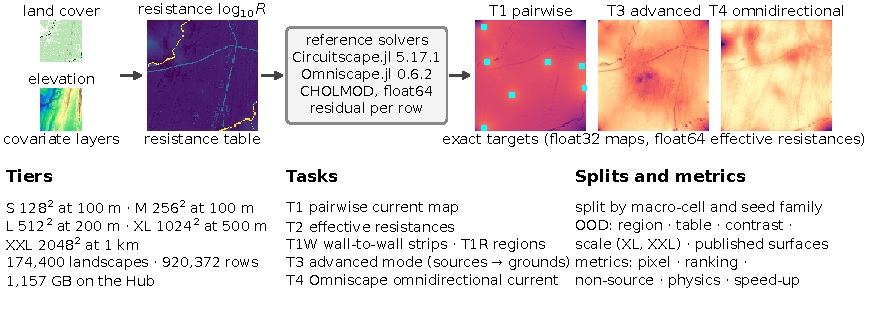
\includegraphics[width=\linewidth]{fig1_overview.pdf}
  \caption{AmpScape in one view. Open covariate layers (or a synthetic generator) and a resistance table give a resistance raster; the reference solvers produce exact pairwise, advanced-mode and omnidirectional current maps, which the tasks turn into learning targets. Five tiers, the task menu, the split design and the metric families are listed below the pipeline.}
  \label{fig:overview}
\end{figure}

\paragraph{Contributions.} (i)~\emph{The dataset}: 174,400 landscapes on five tiers from $128^2$ at 100~m to $2048^2$ at 1~km, 60\,\% synthetic with a hard-case stratum and 40\,\% real tiles from open global layers, each solved under five resistance tables (Figure~\ref{fig:overview}, Table~\ref{tab:counts}). (ii)~\emph{A reference-solver protocol with measured fidelity}: every pairwise and advanced-mode row carries its Kirchhoff residual, and the block-centred Omniscape targets are measured against exact block-1 references (mean \relltwo{} 0.029 at M, 0.028 at L) that become the official evaluation surface at those tiers. (iii)~\emph{A harness} with pixel, ranking, non-source-pixel, physics and efficiency metrics, a framework-agnostic prediction format and a leaderboard. (iv)~\emph{Baselines}: five model families, three seeds, configurations tuned per tier and selected per task on validation loss alone, with scale-transfer, OOD, data-scaling and solver-acceleration studies. (v)~\emph{A many-query demonstration} on a 160-map screening study.
% src: docs/dataset_card.md; docs/t4_fidelity.md; docs/wp7_demo.md

The headline is a trade-off, not a replacement. On the omnidirectional task the best surrogate reaches \relltwo{} 0.041, 0.042 and 0.081 at S, M and L at median speed-ups of 167,020$\times$, 32,789$\times$ and 111,998$\times$ over the production solver; against the exact map it sits at 0.051 (M) and 0.090 (L) where the production block solver sits at 0.029 and 0.032. Pairwise current is harder for every model (best \relltwo{} 0.114 / 0.187 / 0.299), zero-shot transfer to XL and XXL fails on magnitude by exactly the factor the larger window injects (\relltwo{} $\approx 0.50$ and $\approx 0.75$, Appendix~\ref{app:derivation}), and ranking metrics survive where magnitudes do not.
% src: paper/tables/baselines_sml.md; paper/tables/t4_pareto_M.md; paper/tables/t4_pareto_L.md; derived: 1 - 64/128 and 1 - 64/256 from docs/t4_fidelity.md

\section{Related work}
\label{sec:related}

\paragraph{Circuit theory as ground truth, and its cost.} McRae's isolation by resistance \citep{mcrae2006} and its connectivity tool \citep{mcrae2008} solve Kirchhoff's equations on the raster graph; Circuitscape.jl uses CG+AMG and CHOLMOD solvers \citep{anantharaman2020,hall2021}, Omniscape applies it in a moving window around every source pixel \citep{mcrae2016,landau2021}, gflow parallelises pairwise solves \citep{leonard2017}, ConScape covers the randomised-shortest-path continuum \citep{vanmoorter2023,panzacchi2016}, and current density has been computed at global extent \citep{brennan2022}. Nearly-linear-time solvers \citep{koutis2010} and effective-resistance sketches \citep{spielman2011} exist in theory, but production workloads use CG+AMG or CHOLMOD, and because resistance surfaces are uncertain \citep{zeller2012} they are called repeatedly \citep{peterman2018,hanks2013,bowman2020}. The practitioner literature records the omnidirectional cost---``55 CPUs and 350 GB RAM (approximately 140 h)'' per species, ``a level of high-throughput computing capacity likely not available to most conservation practitioners'' \citep{dertien2023}; 196~h for a regional 30~m run \citep{heckford2026}---and the standard mitigation, \code{block\_size}, is documented as giving ``only negligable [sic] differences'' \citep{omniscapedocs} and set to 10\,\% of the window radius in practice \citep{belote2022}; AmpScape measures this approximation against exact block-1 solutions (Section~\ref{sec:data}).
% src: paper/sections/related_work.md

\paragraph{Where to intervene, and ML for connectivity.} Barrier Mapper \citep{mcrae2012}, Pinchpoint Mapper \citep{linkagemapper}, Zonation \citep{moilanen2005,moilanen2022}, Marxan Connect \citep{daigle2020} and GECOT \citep{hamonic2025} prioritise interventions; analytical sensitivities \citep{vanmoorter2026} and differentiable, GPU-accelerated distances \citep{boussange2025} show that exact solvers are differentiable and accelerator-capable, so the case for a surrogate is amortised cost across many queries. Machine learning has been used \emph{around} connectivity \citep{equihua2024,smith2023}, but our searches found no learned surrogate of Circuitscape or Omniscape and no public benchmark of solver-computed circuit-theory outputs.

\paragraph{Learned surrogates for elliptic problems; benchmark design.} Circuitscape's system discretises $\nabla\cdot(\sigma\nabla\phi)=f$ with point sources and grounds, so the closest lineage is operator learning on Darcy flow---FNO \citep{li2021}, PDEBench \citep{takamoto2022}, the neuraloperator library \citep{kossaifi2024}, U-Net baselines \citep{ronneberger2015,gupta2022}, graph networks \citep{battaglia2018,pfaff2021}---with multiscale, high-contrast coefficients as the recognised hard case \citep{liu2024,he2024,xu2024,haltmayer2026,trifonov2024} and learned preconditioners that accelerate rather than replace the solver \citep{lan2024,li2023}. The delta is in the data: the standard Darcy-rough coefficient has ``a contrast of 6'' with ``$f(x)\equiv 1$'' \citep{xu2024}, whereas AmpScape has real coefficient fields, contrast up to $10^6$, per-sample singular sources, grids to $2048^2$, systematic OOD splits and decision-relevant metrics. The release follows PGLearn \citep{klamkin2025} and OPFData / OPF-Learn \citep{lovett2024,joswigjones2021}---reference solver, instance families, complete solutions, Hub hosting---PDEBench, The Well and AirfRANS for uniform HDF5 shards, cards and explicit OOD tasks \citep{ohana2024,bonnet2022}, and Datasheets for Datasets and the track call for documentation and Croissant \citep{gebru2021,neurips2026cfp}.
% src: paper/sections/related_work.md

\section{Problem and tasks}
\label{sec:tasks}

Each sample pairs a resistance raster $R$ ($H\times W$, $R\ge 1$, NoData masked) and a source configuration with the exact output of Circuitscape.jl 5.17.1 or Omniscape.jl 0.6.2: one node per valid pixel, 8-neighbour edges of conductance $g_{ij}=(g_i+g_j)/2$ with $g=1/R$, voltages $v$ solving $Lv=b$ for the injection vector $b$, and Circuitscape's node current density as the stored map. The reference solver is CHOLMOD in double precision, every sample records its residual $\|Lv-b\|_2/\|b\|_2$, and outputs are stored raw (float32 maps, float64 effective resistances).
% src: docs/task_specification.md

\textbf{T1, pairwise current}: Circuitscape \code{pairwise} mode with $K\in[2,8]$ single-pixel focal nodes and all $K(K-1)/2$ pairs (node $i$ grounded, 1~A injected at node $j$); target \code{cum\_current} ($H\times W$), with the $K\times K$ effective-resistance matrix as the \textbf{T2} target. \textbf{T1W} uses $K=2$ edge strips as focal regions (strip pixels excluded from the metrics), \textbf{T1R} habitat patches as short-circuited regions. \textbf{T3}, advanced mode: source raster values are injected currents and grounds are ideal; targets \code{current} and \code{voltage}. \textbf{T4}, omnidirectional connectivity: Omniscape grounds in turn every pixel with source strength above \code{source\_threshold} (= 0) on a grid of stride \code{block\_size}, injects current $\propto S$ from all sources within \code{radius} px and sums the window maps (sources: inverse-resistance suitability above the 0.5 quantile, rescaled to a maximum of 1). Production radius~/ block per tier: S 16~/ 1, M 32~/ 3, L 64~/ 5, XL 128~/ 11, XXL 256~/ 25 px (block = largest odd integer $\le$ radius/10), \code{correct\_artifacts = true}; block 1 is exact, larger blocks give the block-centred map, a measured approximation (Section~\ref{sec:data}).
% src: docs/task_specification.md; configs/tasks/sources_default.yaml; docs/t4_fidelity.md

\textbf{Inputs and target for learning.} Baselines receive standardised log-resistance (train-only statistics, 0 at NoData), the NoData mask and the task's source channels (T1 focal mask; T3 scaled source strength and ground mask; T4 Omniscape source strength), and predict $\log_{10}(C+\epsilon\cdot\max C)$, $\epsilon=10^{-6}$, under a masked MSE; the $\epsilon$-shifted log is scale-invariant and bounds the dynamic range to 6 decades below the map maximum.
% src: ampscape/models/common.py; ampscape/metrics/transforms.py

\section{The dataset}
\label{sec:data}

% src: docs/tables/final_counts.json; docs/dataset_card.md
\begin{table}[tb]
\centering
\footnotesize
\setlength{\tabcolsep}{3.5pt}
\caption{AmpScape v1.0 per tier. A landscape is one resistance raster; each of its source configurations is a configuration row. The 25 rows failing quality control (24 landscapes, all synthetic at contrast $\geq 10^4$) stay in the index with their flags and are excluded from the split lists.}
\label{tab:counts}
\begin{tabular}{llrrrrr}
\toprule
tier & raster $\cdot$ pixel & landscapes & configuration rows & synthetic / real & GB on the Hub & rows failing QC \\
\midrule
S & 128$^2$ $\cdot$ 100 m & 100,000 & 527,281 & 60,000 / 40,000 & 142.4 & 1 \\
M & 256$^2$ $\cdot$ 100 m & 50,000 & 264,128 & 30,000 / 20,000 & 251.7 & 4 \\
L & 512$^2$ $\cdot$ 200 m & 20,000 & 105,949 & 12,000 / 8,000 & 380.9 & 11 \\
XL & 1024$^2$ $\cdot$ 500 m & 4,000 & 21,006 & 2,400 / 1,600 & 281.7 & 7 \\
XXL & 2048$^2$ $\cdot$ 1 km & 400 & 2,008 & 210 / 190 & 100.7 & 2 \\
total &  & 174,400 & 920,372 &  & 1157.4 & 25 \\
\bottomrule
\end{tabular}
\end{table}


\paragraph{Landscapes.} A landscape is one resistance raster; each of its source configurations is a configuration row (Table~\ref{tab:counts}). \emph{Real landscapes} are covariate stacks from ESA WorldCover, Copernicus DEM, GRIP4 roads, HydroRIVERS and gHM (13\,958 tiles, 69\,790 resistance rasters); each tile yields five landscapes, one per resistance table---four expert-style tables and one seeded random table per tile, with the \code{forest\_bird} table ($r_{\max}$ 100 versus 1000) held out. Class ordering and term structure follow the literature; the numeric values are AmpScape's own, not species-calibrated truth. \emph{Synthetic landscapes} come from neutral landscape models and random fields, with 20\,\% in a hard stratum (contrast $10^5$ and $10^6$, $r_{\max}$-saturated, narrow corridors, large NoData); contrast $10^6$ is reserved for the OOD contrast set (Figure~\ref{fig:gallery}).
% src: CHANGELOG.md; docs/dataset_plan.md; DECISIONS.md; docs/dataset_card.md

\begin{figure}[tb]
  \centering
  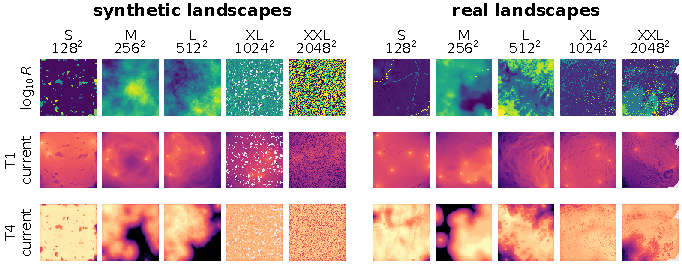
\includegraphics[width=0.6\linewidth]{fig2_gallery.pdf}
  \caption{Data gallery: one synthetic (left) and one real (right) \code{test\_id} landscape per tier---$\log_{10}$ resistance, the T1 pairwise current map and the T4 omnidirectional current map ($\log_{10}$ scale, NoData grey). Rows are S ($128^2$) to XXL ($2048^2$); labels name the generator or the resistance table.}
  \label{fig:gallery}
  % src: docs/dataset_card.md
\end{figure}

\paragraph{Task groups and layout.} Every landscape receives \code{points} (T1), two wall-to-wall strips (T1W), an \code{advanced} configuration (T3) and an Omniscape configuration (T4); landscapes with $\ge 2$ eligible habitat patches also get \code{regions} (T1R). Shards are per tier and task group with a per-tier index (one row per sample $\times$ configuration), split lists and \code{croissant.json}, so any tier or task group downloads alone; four nested shard-prefix subsets---\code{mini} (0.6~GB), \code{lite} ($\approx 26$~GB: 8\,000 S + 2\,400 M + 800 L landscapes), \code{core} (115.5~GB) and \code{full} (1\,157.4~GB)---each have an index column, split lists and a Croissant FileSet. Hosting: \code{Xirro/AmpScape}, CC BY 4.0, Croissant 1.0 with RAI fields; v1.0 is the data revision, v1.0.1 and v1.0.2 metadata-only tags.
% src: docs/dataset_plan.md; docs/dataset_card.md; DECISIONS.md

\paragraph{Reference solver, precision pass, Omniscape fidelity.} All T1/T1W/T1R/T3 targets are computed with the direct CHOLMOD solver in double precision, with the Kirchhoff residual recorded from full-precision voltages (QC threshold $10^{-6}$). A post-run precision pass re-solved every row whose residual was above $10^{-9}$, unmeasured, CG+AMG-solved or QC-failed---129,722 rows---with CHOLMOD on the reduced system plus up to three refinement steps: 3,861 rows remain between $10^{-9}$ and $10^{-6}$ (kept) and 20 rows, all synthetic at contrast $\ge 10^4$, are flagged and excluded from the split lists together with the other QC failures (25 rows, 24 landscapes; Appendix~\ref{app:precision}). T4 targets use Omniscape.jl 0.6.2 with artefact correction. Because \code{block\_size} is part of the method, it is fixed per tier by the rule above and the block-centred approximation is \emph{measured}: on the 1\,000-sample M reference the production block-3 target deviates from the exact block-1 map by mean \relltwo{} 0.029 with 4.7\,\% of samples above 5\,\%; the L target (block 5, 60 samples) by mean 0.028 (max 0.058); block 1 costs 6.7$\times$ (M) and 22$\times$ (L) the production solve. These block-1 references are the official T4 evaluation surface at M and L (Appendix~\ref{app:fidelity}). Generation took 16\,552 core-hours including the precision pass; each tier was audited on the Hub against the plan (sha256, sample ids, configurations, index rows), regeneration on the same CPU model is bitwise reproducible, and across CPU models results differ by $\le 1.2\times 10^{-9}$ relative.
% src: DECISIONS.md; docs/tables/precision_pass.md; docs/dataset_card.md; configs/solver/omniscape_reference.yaml; docs/t4_fidelity.md; docs/tables/dataset_statistics.md; docs/generation_postmortem.md

\section{Splits and out-of-distribution design}
\label{sec:splits}

Splits are assigned by the \emph{unit of leakage}---the tile for real landscapes, the seed family for synthetic ones---at base fractions 0.8~/ 0.1~/ 0.1, with hold-outs applied before the draw. Because an S tile physically sits inside XL/XXL footprints, the globe is partitioned once into 104 equal-width macro-cells with one seeded assignment applied at every tier (70 land cells: 56 train~/ 7 val~/ 7 test\_id); no train/val tile box intersects any test tile box at any tier, XXL stays test-only, seed ranges are tier-disjoint, and 25\,\% of XL landscapes are train/val (counts in Appendix~\ref{app:splits}).
% src: docs/dataset_plan.md; DECISIONS.md; configs/datasets/v1_0.yaml; CHANGELOG.md

\textbf{OOD sets} (one boolean index column each): \code{region}---real tiles in the Montane Grasslands \& Shrublands or Mangroves biomes or the Australasia realm; \code{table}---every landscape built with the \code{forest\_bird} table; \code{contrast}---synthetic contrast $10^6$; \code{scale}---XL/XXL evaluated by models trained at $\le$ L, with a \code{strict} subset of 6 XXL real tiles that overlap no training tile at any tier; \code{synth2real}---a loader flag restricting training to synthetic landscapes; \code{published}---45 S tiles and 1 XXL tile with published resistance surfaces. Held-out-table and held-out-contrast landscapes that the base draw would place in train/val are demoted to \code{test\_ood}. Pixel size, raster size and the T4 window radius co-vary across tiers, so the scale set measures combined scale transfer; XXL footprints overlap finer-tier training cells, so only the strict subset isolates spatial novelty as well as resolution.
% src: configs/datasets/v1_0.yaml; docs/dataset_card.md; ampscape/splits/assign.py

\section{Metrics and evaluation protocol}
\label{sec:metrics}

Maps are compared in $\log_{10}(C+\epsilon\cdot\max C)$. \emph{Pixel}: MAE in $\log_{10}$-$\epsilon$ space (primary), MSE and relative L2 on raw values, SSIM/PSNR secondary; NoData and T1W strip pixels masked. \emph{Domain}: top-$q$\,\% IoU of the $q$\,\% highest-current valid pixels ($q\in\{1,5,10\}$); corridor Dice above the 10\,\% quantile; pinch-point recall (target pinch points = local maxima in a $7\times 7$ window within the top 5\,\%, hit = a predicted local maximum within 3~px); Spearman rank correlation---conventions, not validated ecological criteria. \emph{Non-source pixels}: currents are singular at injection pixels, so \relltwo{}, MAE and top-$q$ IoU are also computed outside source, focal and ground pixels plus a 2-px halo. \emph{Physics}: Kirchhoff residual of a predicted voltage, focal-current error, non-negativity, throughput error. \emph{Efficiency}: speed-up = solver wall time~/ inference time, batch 1 at XL/XXL. \emph{Acceleration}: AMG-preconditioned CG iterations and wall time to the reference tolerance from a predicted voltage versus from zero.
% src: ampscape/metrics/transforms.py; ampscape/metrics/pixel.py; ampscape/metrics/domain.py; docs/dataset_card.md; ampscape/metrics/nonsource.py; ampscape/metrics/physics.py; ampscape/metrics/efficiency.py; scripts/transfer_eval.py; ampscape/metrics/acceleration.py

Results are reported on \code{test\_id} and every OOD split, three seeds per configuration (mean $\pm$ sample std), with early stopping on \code{val}. \relltwo{} is additionally reported as the median over seeds: it is a ratio of squared sums dominated by the few highest-current landscapes, so one seed that misses them moves the mean by more than the seed spread of every other metric (at L the three GNN seeds give 0.789, 0.925 and 1.108 while their MAE and Spearman agree within 0.02). Predictions are framework-agnostic (Appendix~\ref{app:format}) and scored by one harness; at M and L the primary T4 metrics are computed against the exact block-1 map on the reference subsets (400~/ 300~/ 300 landscapes per split at M; 24~/ 16~/ 20 at L). The leaderboard on the Hub accepts the same format; entries are validated and appended by a maintainer.
% src: docs/TASK_BRIEF.md; docs/tables/baselines_full.md; ampscape/eval/harness.py; docs/evaluation.md; docs/tables/t4_pareto_M.md; docs/tables/t4_pareto_L.md; DECISIONS.md; docs/submission.md

\section{Baselines and results}
\label{sec:results}

\paragraph{Models, protocol, configuration selection.} All learned baselines share the inputs and target of Section~\ref{sec:tasks}. \textbf{U-Net}: 4-level encoder--decoder, width 32 (7.8~M parameters), tuned width-64 variant \code{w64} (31.0~M). \textbf{FNO}: 64 retained modes plus a distance-to-source channel, width 32 (33.6~M), tuned width-48 variant \code{w48} (75.5~M). \textbf{ViT}: patch-4 embedding, global attention (dim 192, depth 6), a learned $32\times 32$ positional embedding interpolated to other grids (3.0~M); tuned \code{p16g16} variant with patch 16 at M. \textbf{GNN}: grid-as-graph message passing with a $4\times$-coarsened second level (\code{ms}, 0.2~M), tuned $8\times$-coarsened variant \code{ms8}. \textbf{MgNO} \citep{he2024}: the authors' MIT release (0.58~M), seed 1 at S and M on T1 and T4. Non-learned rows: Omniscape \emph{block-size rows} and a coarsen-$\times 4$-and-upsample solve. Each run trains one model on one task at one tier for 30 epochs with AdamW, a cosine schedule, patience 8 and a fixed seed, three seeds per (model, task, tier), with train-only normalisation statistics of the training tier at every evaluation tier. One alternative configuration per model was trained at M and L on T1 (seed 1) and compared on validation loss; the winners were re-trained with three seeds on every task, and the official configuration is chosen \emph{per model $\times$ task $\times$ tier on validation loss alone}---tuned only if its mean best validation loss over seeds beats the pre-tuning mean by more than the pre-tuning standard error (std$/\sqrt{3}$); test metrics are never read and no decision is carried across tasks. Of the fifteen decisions (Appendix~\ref{app:tables}), the tuned configuration is official for FNO w48 at every task at M and L, U-Net w64 at T1 and T4 M, ViT p16g16 at T1 M and GNN ms8 at T1 M, T1 L and T4 L; the pre-tuning configuration stays official for U-Net T3 M ($-1.4$\,\%, inside the seed spread), ViT T4 M ($+16.8$\,\%) and GNN T4 M ($+8.0$\,\%), and at L no U-Net or ViT candidate beat the official one. Everything learned consumed 701.5 GPU-hours across 773 jobs.
% src: ampscape/models/unet.py; ampscape/models/fno.py; ampscape/models/vit.py; ampscape/models/gnn.py; docs/tables/tuning_full.md; docs/wp6_implementations.md; paper/tables/baselines_sml.md; ampscape/models/coarsen.py; docs/tables/t4_pareto_M.md; scripts/train.py; docs/phase10_full_schedule.md; scripts/transfer_eval.py; docs/tables/tuning_decisions.md; docs/tables/gpu_usage.md

% src: paper/tables/baselines_sml.md
\begin{table}[tb]
\centering
\scriptsize
\setlength{\tabcolsep}{3.5pt}
\caption{Relative L2 on \texttt{test\_id} at the training tier, mean $\pm$ std over three seeds with the median over seeds in brackets (official configuration per model $\times$ task $\times$ tier; MgNO: three seeds at S and M, not ranked because 4 of its 6 T4 runs diverged, see text). Best three-seed model per task and tier in bold; lower is better. The complete metric set (MAE, top-5\,\% IoU, pinch recall, Spearman, speed-up, training cost) is Table~\ref{tab:baselines_full}.}
\label{tab:results}
\begin{tabular}{llccc}
\toprule
task & model & S & M & L \\
\midrule
T1 & U-Net & \textbf{0.114 $\pm$ 0.007 [0.111]} & \textbf{0.187 $\pm$ 0.022 [0.187]} & 0.397 $\pm$ 0.011 [0.392] \\
T1 & FNO & 0.199 $\pm$ 0.002 [0.199] & 0.208 $\pm$ 0.003 [0.209] & \textbf{0.299 $\pm$ 0.011 [0.297]} \\
T1 & ViT & 0.218 $\pm$ 0.028 [0.229] & 0.306 $\pm$ 0.013 [0.299] & 0.648 $\pm$ 0.033 [0.644] \\
T1 & GNN & 0.561 $\pm$ 0.005 [0.563] & 0.607 $\pm$ 0.027 [0.600] & 0.941 $\pm$ 0.160 [0.925] \\
T1 & MgNO & 0.444 $\pm$ 0.238 [0.419] & 0.376 $\pm$ 0.044 [0.389] & -- \\
T3 & U-Net & \textbf{0.111 $\pm$ 0.005 [0.110]} & \textbf{0.202 $\pm$ 0.005 [0.202]} & 0.379 $\pm$ 0.012 [0.374] \\
T3 & FNO & 0.252 $\pm$ 0.001 [0.252] & 0.255 $\pm$ 0.003 [0.254] & \textbf{0.323 $\pm$ 0.002 [0.323]} \\
T4 & U-Net & \textbf{0.041 $\pm$ 0.001 [0.041]} & \textbf{0.042 $\pm$ 0.001 [0.041]} & \textbf{0.081 $\pm$ 0.001 [0.081]} \\
T4 & FNO & 0.051 $\pm$ 0.001 [0.051] & 0.073 $\pm$ 0.000 [0.073] & 0.116 $\pm$ 0.000 [0.116] \\
T4 & ViT & 0.052 $\pm$ 0.001 [0.052] & 0.094 $\pm$ 0.004 [0.093] & 0.159 $\pm$ 0.004 [0.161] \\
T4 & GNN & 0.066 $\pm$ 0.000 [0.066] & 0.099 $\pm$ 0.001 [0.099] & 0.142 $\pm$ 0.001 [0.142] \\
T4 & MgNO & 0.358 $\pm$ 0.544 [0.045] & 0.184 $\pm$ 0.021 [0.189] & -- \\
\bottomrule
\end{tabular}
\end{table}


\paragraph{In-distribution results.} Table~\ref{tab:results} and Figure~\ref{fig:error_vs_tier} give \relltwo{} on \code{test\_id}; Figure~\ref{fig:qualitative} shows the best T1 and T4 models at L on an in-distribution and an out-of-distribution landscape. First, the task families differ: T4 is the easier learning problem and the one with the real compute problem---the U-Net stays at \relltwo{} 0.041--0.081 from S to L with Spearman 0.996~/ 0.996~/ 0.991 at median speed-ups of 167,020$\times$~/ 32,789$\times$~/ 111,998$\times$ over the production Omniscape run---whereas T1 and T3, globally coupled through one sparse solve, are harder for every model and give speed-ups of only $10^2$--$10^3$ (U-Net T1 625$\times$~/ 537$\times$~/ 691$\times$) because a full-raster pairwise solve is already cheap. Second, error grows with tier for every model and task (best T1 0.114 at S to 0.299 at L; best T4 0.041 to 0.081). Third, ranking metrics degrade more slowly than magnitudes: between S and L the T4 U-Net's \relltwo{} doubles (0.041 $\rightarrow$ 0.081) and its pinch-point recall drops from 0.918 to 0.825 while its Spearman moves from 0.996 to 0.991.
% src: paper/tables/baselines_sml.md

\begin{figure}[tb]
  \centering
  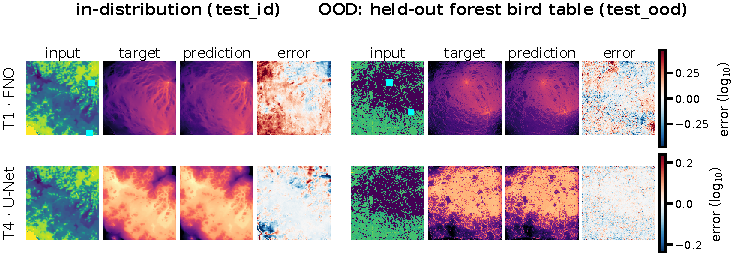
\includegraphics[width=0.5\linewidth]{fig3_qualitative.pdf}
  \caption{Qualitative results at L for the official T1 model (FNO w48) and T4 model (U-Net) on a real \code{test\_id} landscape and a \code{test\_ood} landscape built with the held-out \code{forest\_bird} table: input $\log_{10}R$ with the focal nodes, exact target, prediction and the error in $\log_{10}$ units. Pairwise errors concentrate along the long-range flow paths; omnidirectional errors are local and small except at the NoData boundary.}
  \label{fig:qualitative}
\end{figure}

The families fail in different places. The U-Net is strongest on T1 and T4 at S and M but loses its T1 lead to the FNO at L (0.397 vs 0.299); the FNO has the best T1 result at L, the highest T1 Spearman at every tier and the best transfer (below); the ViT is competitive at S (T1 0.218, T4 0.052) and resolution-inappropriate at L even after tuning (T1 0.648, top-5\,\% IoU 0.146); the GNN is far behind on T1 (0.561~/ 0.607~/ 0.941) but competitive on the locally windowed T4 (0.066~/ 0.099~/ 0.142) at 5.06--9.44 GPU-h per run against 0.79--1.97 for the U-Net; MgNO (seed 1) matches the U-Net on T4 at S (0.044 vs 0.041) but falls to 0.189 at M and 0.220~/ 0.412 on T1. No family wins on accuracy, scale robustness, OOD robustness and cost at once; that trade-off is the result.
% src: paper/tables/baselines_sml.md

\begin{figure}[b]
  \centering
  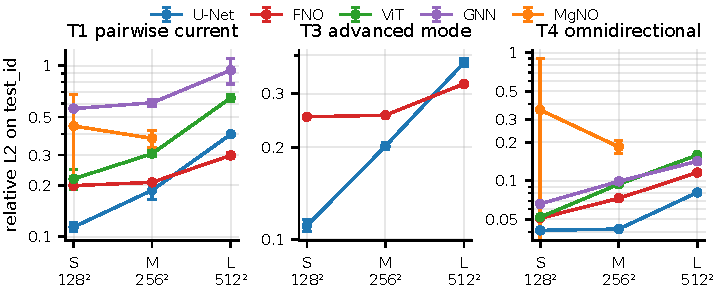
\includegraphics[width=\linewidth]{fig4_error_vs_tier.pdf}
  \caption{Relative L2 on \code{test\_id} versus training tier per task and model (mean $\pm$ std over three seeds; MgNO one seed). Error grows with tier for every model and task; the ordering of the families differs between the globally coupled pairwise and advanced-mode tasks and the locally windowed omnidirectional task.}
  \label{fig:error_vs_tier}
\end{figure}

\paragraph{T4 against the exact reference.} For the reference subsets we computed exact block-1 maps, so solver approximations and learned models share one error-versus-cost axis (Figure~\ref{fig:pareto}; rows in Appendix~\ref{app:tables}). The production targets approximate the exact map well (\relltwo{} 0.0291 at M, 0.0315 at L), so a model's error against its training target and against the exact map differ little (U-Net 0.042 vs 0.0510 at M, 0.081 vs 0.0903 at L); Omniscape's artefact correction matters more than the block size (block 3 without correction, 0.1105, is worse than block 7 with it, 0.0983, at M); and the learned models occupy a different part of the frontier rather than dominating it: at M the U-Net's 0.0510 lies between the production solver (0.0291 at 111~s) and block 7 (0.0983 at 25.5~s) at 0.00328~s per landscape, at L its 0.0903 matches block 11 (0.0854 at 164~s) at 0.00652~s. Whoever needs \relltwo{} $<0.03$ still needs the solver; whoever needs hundreds of maps at $\approx 0.05$--$0.09$ does not.
% src: paper/tables/t4_pareto_M.md; paper/tables/t4_pareto_L.md; paper/tables/baselines_sml.md

\begin{figure}[tb]
  \centering
  \begin{minipage}[t]{0.48\linewidth}
    \centering
    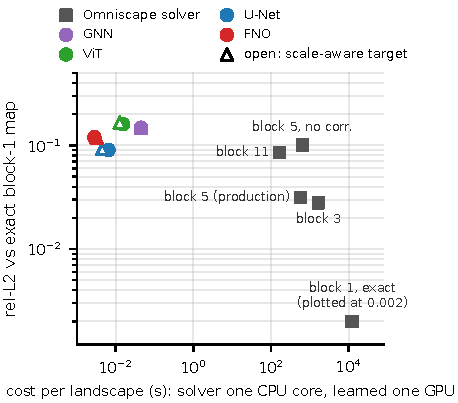
\includegraphics[width=\linewidth]{fig5_pareto_L.pdf}
    \caption{T4 at L: error against the exact block-1 map on the \code{test\_id} reference subset versus cost per landscape (solver rows: one CPU core; learned rows: GPU inference, seeds averaged). Block 1 has error 0 and is plotted at 0.002.}
    \label{fig:pareto}
    % src: derived: plotting position of the exact row in fig5
  \end{minipage}\hfill
  \begin{minipage}[t]{0.48\linewidth}
    \centering
    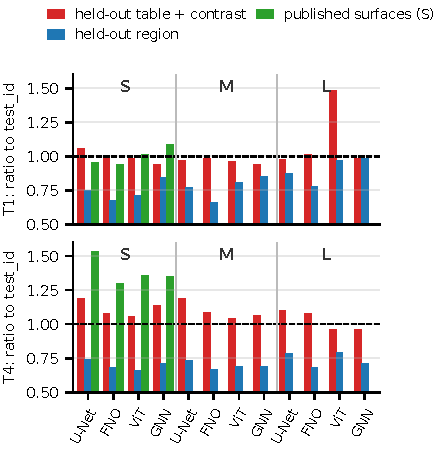
\includegraphics[width=\linewidth]{fig7_ood.pdf}
    \caption{Per-split OOD degradation at the training tier for T1 and T4 (T3 in Appendix~\ref{app:tables}): \relltwo{} on each split divided by \relltwo{} on \code{test\_id} (mean over three seeds). Ratios above 1 are degradation; the held-out region split is easier by composition.}
    \label{fig:ood}
  \end{minipage}
\end{figure}

\paragraph{Scale transfer.} Models trained at L were evaluated at XL ($1024^2$) and XXL ($2048^2$) without fine-tuning, with the official configuration (zero-shot, three seeds) and with a variant whose training target is divided by a factor computed from the inputs and the evaluation tier only---the Omniscape radius ratio $r_L/r_{\mathrm{tier}}$ for T4, $\sqrt{N_{\mathrm{valid}}/512^2}$ for T1 (scale-aware, seed 1); the ViT's interpolated positional embedding stops at XL (Figure~\ref{fig:scale}). Zero-shot transfer fails on magnitude in a regular way for T4: every model lands at \relltwo{} 0.498--0.538 at XL and 0.739--0.764 at XXL, which equals $1-r_L/r_{\mathrm{tier}}$, the share of the current that the larger Omniscape radius adds and an L-trained model cannot know about (Appendix~\ref{app:derivation}: 0.50 and 0.75). Removing that factor recovers T4 to 0.157--0.308 at XL and 0.197--0.438 at XXL, still above in-tier errors but no longer set by a known factor; the FNO transfers best (0.157~/ 0.197). For T1 the scale-aware target helps the FNO at XXL (1.352 $\rightarrow$ 0.762) but not at XL (0.617 $\rightarrow$ 0.700), the U-Net stays near \relltwo{} 1 (0.957~/ 0.987)---its receptive field, not the magnitude, is the limit---and the GNN variant diverges at XL (7.509). Rankings survive what magnitudes do not: the zero-shot T4 U-Net keeps Spearman 0.992~/ 0.946~/ 0.904 at L~/ XL~/ XXL while its \relltwo{} goes 0.081 $\rightarrow$ 0.515 $\rightarrow$ 0.749; the one unstable case is the zero-shot T1 U-Net at XXL (4.425 $\pm$ 3.659, Spearman 0.461 $\pm$ 0.034). A surrogate trained at one resolution can still \emph{rank} locations at a larger one, but its absolute currents must be rescaled or re-trained.
% src: paper/tables/scale_transfer.md; ampscape/models/common.py; docs/phase10_full_schedule.md; derived: 1 - 64/128 and 1 - 64/256 from docs/t4_fidelity.md

\begin{figure}[tb]
  \centering
  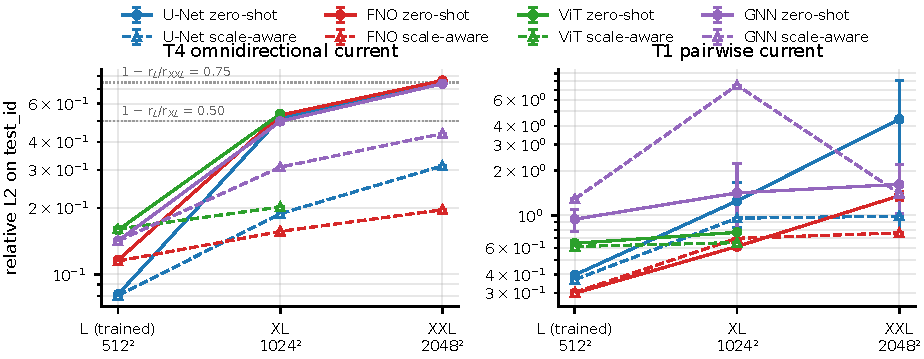
\includegraphics[width=\linewidth]{fig6_scale_transfer.pdf}
  \caption{Scale transfer of L-trained models to XL and XXL on \code{test\_id}: zero-shot (solid, three seeds) versus the scale-aware target (dashed, seed 1). The dotted lines in the T4 panel mark $1-r_L/r_{\mathrm{tier}}$, the magnitude the larger Omniscape window adds.}
  \label{fig:scale}
\end{figure}

\paragraph{Out-of-distribution degradation.} Figure~\ref{fig:ood} gives \relltwo{} on the in-tier OOD splits relative to \code{test\_id} (values in Appendix~\ref{app:tables}). A held-out resistance table and contrast cost little at the training tier: the \code{test\_ood} ratio is 0.920--1.200 for every model, task and tier except the ViT on T1 at L (1.486, its structurally failing configuration); T4 is the most sensitive family (1.039--1.200). Published real resistance surfaces are the hardest in-tier set for T4 (S only: ratios 1.273--1.524) while T1 and T3 stay within 0.941--1.145 of \code{test\_id}; since T4 surrogates are the ones that would run on practitioners' own surfaces, this is the number to quote beside the headline. The held-out-region split is \emph{easier} than \code{test\_id} for every model, task and tier (ratios 0.655--0.982), which is not evidence of spatial robustness: the split is real-tile only and the held-out biomes differ in composition (at S a p90 contrast of 595 against 10,000 for \code{test\_id}); errors track landscape difficulty more than spatial novelty, so \code{ood\_region} is a spatial-leakage control, not a stress test.
% src: paper/tables/ood_degradation.md; paper/ood_analysis.md

\paragraph{Data scaling and solver acceleration.} U-Net and FNO were trained on T1 at S with 1,000, 5,000 and 20,000 landscapes for 30 epochs or for the official run's optimisation steps (seed 1), against the official run on 61,577 landscapes (Appendix~\ref{app:tables}). At a fixed step budget the U-Net saturates early (20,000 landscapes give 0.103 and 5,000 give 0.139 against 0.111 for the full run), so the 30-epoch protocol at S is budget-limited rather than data-limited for the U-Net, whereas the FNO keeps improving with data (0.438 $\rightarrow$ 0.298 $\rightarrow$ 0.246 $\rightarrow$ 0.198); fixed-epoch training on small subsets understates both, so the regime must be stated when quoting data efficiency. For T1--T3 the practically relevant question is whether a predicted voltage shortens the exact solve: U-Net and FNO voltage heads (T3 and the first pair of each T1 landscape, seed 1) warm-started the reference solver's AMG-preconditioned CG on every \code{test\_id} and \code{test\_ood} system at S, M and L, to a relative residual of $10^{-6}$. There is no gain anywhere (T3 \code{test\_id}, U-Net start: 10 $\rightarrow$ 10 iterations at S, 12 $\rightarrow$ 13 at M, 17 $\rightarrow$ 19 at L): the predicted maps are accurate in the MAE sense but their relative Kirchhoff residual is 82.5 to $3.87\times 10^{3}$ times that of the zero vector---a pixel-wise error of a few per cent is high-frequency, the Laplacian amplifies it, and PCG removes it in the same iterations it needs from zero. The value of the surrogates on these tasks is the cheaper \emph{map}, not a better initial guess.
% src: paper/tables/wp4_data_scaling.md; docs/tables/acceleration.md

\section{Many-query demonstration}
\label{sec:wp7}

The case for a T4 surrogate is the study that needs many maps per landscape. We ran the best T4 model at L (U-Net, seed 1; \relltwo{} 0.080 against the exact block-1 map) on 20 held-out real L tiles $\times$ 8 resistance tables, 160 maps, and asked whether the study-level conclusions drawn from the surrogate match those drawn from the solver (per-tile panels in Appendix~\ref{app:wp7}). Every conclusion is reproduced: the stability of the top-5\,\% regions across tables is 0.458 against the solver's 0.463 (mean pairwise IoU), the consensus core (top 5\,\% in $\ge 75$\,\% of tables) overlaps at IoU 0.825, the ranking of tables by their effect has Spearman 0.991 with the same most-influential table on every tile, and persistent pinch points ($\ge 50$\,\% of tables) are recovered with recall 0.941---at 11.8~s on one GPU against 36.3 CPU-h, i.e.\ 11077$\times$ after training once. The weak point is pinch-point \emph{precision}, 0.657 at 3~px: the surrogate proposes more persistent pinch points than the solver confirms, so a candidate list drawn from it should be solver-verified before it becomes a decision map.
% src: docs/wp7_demo.md

\section{Limitations, ethics and maintenance}
\label{sec:limitations}

\textbf{Limitations.} (1)~Resistance tables are structural proxies, not ecological truth, and a faster approximation does not reduce resistance-surface uncertainty---it lets a user explore it. (2)~Learned models degrade on published surfaces and across scale; final decision maps should be solver-verified. (3)~T4 targets carry a quantified blocking approximation (mean \relltwo{} 0.029 at M, 0.028 at L); at XL/XXL only the production target exists. (4)~Pixel size, raster size and the Omniscape radius are confounded in the scale split, and T4 scale transfer also crosses an operator change (block 5 $\rightarrow$ 11 $\rightarrow$ 25); XXL footprints overlap finer-tier training cells, so only the strict scale subset isolates spatial novelty. (5)~The held-out-region split is a leakage control, not a stress test. (6)~The ViT's official configuration is resolution-inappropriate above S. (7)~The scale-aware variants, the data-scaling ablation, MgNO and the demonstration are single-seed. (8)~Domain-metric thresholds are not validated against ecological outcomes. (9)~Not yet tested: training at XL, fixed-step training at M/L, MgNO at L with three seeds, the resolution-versus-size probe set under \code{aux/}.
% src: docs/dataset_card.md; paper/tables/ood_degradation.md; docs/t4_fidelity.md; paper/ood_analysis.md; DECISIONS.md; paper/tables/scale_transfer.md; paper/tables/wp4_data_scaling.md; docs/wp7_demo.md

The paper does not claim that Circuitscape is slow (a pairwise solve takes seconds at every tier; the documented cost is omnidirectional and many-query), that exact solvers are not differentiable \citep{vanmoorter2026,boussange2025}, or that there is no prior work on where to intervene \citep{mcrae2012,moilanen2022,daigle2020,hamonic2025}.
% src: docs/tables/dataset_statistics.md

\textbf{Ethics, intended use, maintenance.} No personal data: real tiles derive from public land-cover and terrain products at $\ge 100$~m, and no protected-area polygons are used. Every stored covariate comes from a source whose licence permits redistribution of derived rasters (Appendix~\ref{app:licences}); GRIP4 is CC0 by its publisher and CC BY 4.0 in secondary catalogues, so we attribute under the stricter reading. Intended use is screening, not final decisions. Maintenance: versioned Hub revisions, a changelog and decision log, scripted regeneration from the frozen pipeline tag, CI with a licence-consistency test, issues on GitHub, and a DOI minted at acceptance.
% src: docs/dataset_card.md; docs/licenses.md; CHANGELOG.md

\textbf{Reproducibility.} Data on the Hugging Face Hub (\code{Xirro/AmpScape}, CC BY 4.0) with per-tier indexes, split lists, Croissant metadata and per-sample solver provenance; code (MIT) with a locked environment, solver wrapper, generation driver, harness, training and transfer scripts and leaderboard tooling; every figure and table is regenerated by script from the published result files, every number in the text is tagged with its source file and checked by script, and the datasheet and generation post-mortem are in the repository. Compute: 16\,552 CPU core-hours for generation and the precision pass; 701.5 GPU-hours (773 jobs on L40S, A100, H100 and H200 GPUs) for everything learned, including tuning candidates, abandoned legs and duplicates.
% src: docs/generation_postmortem.md; docs/tables/gpu_usage.md; docs/tables/gpu_usage_tuning.md

\bibliographystyle{plainnat}
{\small\bibliography{references}}

\newpage
\appendix

\section{Why zero-shot T4 scale transfer fails by $1-r_{\mathrm{train}}/r_{\mathrm{eval}}$}
\label{app:derivation}

Facts used: Omniscape window radius per tier $r$ = 16, 32, 64, 128 and 256 px for S, M, L, XL and XXL with block size $b$ = largest odd integer $\le r/10$; source strength $s(x)\in[0,1]$ = inverse-resistance suitability above its 0.5 quantile rescaled to a maximum of 1 per landscape; targets are cumulative current summed over windows; measured zero-shot errors of the L-trained models on \code{test\_id}: \relltwo{} 0.515~/ 0.531~/ 0.538~/ 0.498 (U-Net~/ FNO~/ ViT~/ GNN) at XL and 0.749~/ 0.764~/ 0.739 (U-Net~/ FNO~/ GNN) at XXL, three seeds each with std $\le 0.003$.
% src: docs/t4_fidelity.md; paper/tables/scale_transfer.md

\paragraph{Magnitude scales with the window radius.} Omniscape visits every block centre $t$ and solves one circuit per visit: every pixel $x$ within distance $r$ of $t$ injects a current proportional to $s(x)$ and $t$ is grounded; the per-visit maps are summed into the cumulative current $C$. (1)~The injected current per visit is $\sum_{|x-t|\le r}s(x)\approx \bar s\,\pi r^2$, with $\bar s$ the mean source strength of the window (an input the model sees, independent of the tier). (2)~Within one visit the injected current flows towards the single grounded target; for a pixel at distance $\rho$ from $t$ the current crossing a front of length $\propto\rho$ is $\propto \bar s\rho^2/\rho=\bar s\rho$, of order $\bar s r$ over most of the window; the resistance-dependent proportionality constant is what the surrogate learns and its dependence on $r$ is the same for every pixel. (3)~The number of visits covering a pixel is the number of block centres within distance $r$, $\propto (r/b)^2$, a constant ($\approx 100$) under the block rule. Hence $C(y)\propto \bar s\cdot r\cdot g(y)$, where $g$ collects the resistance-dependent, tier-independent factors: doubling the radius doubles the cumulative current to first order.
% src: derived: b = r/10 from docs/t4_fidelity.md

\paragraph{The zero-shot error.} A model trained at L learns $C_L\propto r_L\,\bar s\, g$. Evaluated at radius $r_{\mathrm{eval}}$ on a landscape with the same resistance statistics it predicts $P\approx C_{\mathrm{eval}}\,(r_L/r_{\mathrm{eval}})$: the same $g$, the wrong magnitude. With $\kappa=r_L/r_{\mathrm{eval}}$,
\[\text{\relltwo{}}=\frac{\|P-C_{\mathrm{eval}}\|_2}{\|C_{\mathrm{eval}}\|_2}=\frac{\|(\kappa-1)C_{\mathrm{eval}}+\varepsilon\|_2}{\|C_{\mathrm{eval}}\|_2}\approx 1-\kappa,\]
where $\varepsilon$ is the model's intrinsic error (its in-tier \relltwo{} is 0.081--0.159) and the approximation holds when $(1-\kappa)\|C\|$ dominates $\|\varepsilon\|$. Predicted: XL $1-64/128=0.50$, XXL $1-64/256=0.75$; measured 0.498--0.538 and 0.739--0.764, the small excess accounted for by $\varepsilon$ in quadrature. The near-identical values across four architectures with std $\le 0.003$ across seeds are consistent with an error set by the operator, not the model. Rank metrics ignore a common factor, which is why Spearman stays at 0.894--0.958 at XL while \relltwo{} collapses.
% src: paper/tables/baselines_sml.md; paper/tables/scale_transfer.md; derived: 1 - 64/128 and 1 - 64/256 from docs/t4_fidelity.md

\paragraph{The scale-aware target.} The variant trains on $k\cdot C$ with $k=r_{\mathrm{ref}}/r_{\mathrm{tier}}$, $r_{\mathrm{ref}}=64$, so the regression target $k\cdot C\propto r_{\mathrm{ref}}\,\bar s\,g$ is tier-independent; at evaluation the prediction is divided by $k_{\mathrm{eval}}$, restoring $C_{\mathrm{eval}}\propto r_{\mathrm{eval}}\,\bar s\,g$. No quantity of the evaluation tier other than its radius (a protocol constant) enters, and no XL/XXL data is used in training or in the inverse. What remains is the error that is not a common factor: 0.157--0.308 at XL and 0.197--0.438 at XXL against in-tier 0.081--0.159---the operator-learning transfer error proper, since $b$ and $r$ both scale and the resistance field has a different pixel size and extent. For a pairwise solve a unit current is injected per source regardless of landscape size; under a uniform rescaling by $s$ per axis the current crossing any front spreads over $\propto s$ pixels, so the per-pixel current $\propto 1/s$ while the valid pixel count $N\propto s^2$; $k=\sqrt{N_{\mathrm{valid}}/N_{\mathrm{ref}}}$ with $N_{\mathrm{ref}}=512^2$ makes $k\cdot C$ invariant and is computed from the input mask alone. The measured throughput error of the zero-shot T1 transfers (0.434--0.985 at XL) is the signature of the same mismatch; the correction helps the FNO at XXL (1.352 $\rightarrow$ 0.762) but not the U-Net (0.957~/ 0.987 at XL~/ XXL), whose receptive field does not cover the longer flow paths of larger landscapes. The argument assumes $b/r$ fixed by the block rule, sources with tier-independent mean strength, the same resistance statistics across tiers (real XL/XXL tiles have coarser pixels than L, part of the residual) and windows that fit inside the landscape for most pixels; it explains the magnitude of the zero-shot error and does not predict which model transfers best once the magnitude is corrected.
% src: ampscape/models/common.py; paper/tables/scale_transfer.md; paper/tables/baselines_sml.md

\section{Full result tables}
\label{app:tables}

Every table is generated by \code{scripts/paper\_tables\_tex.py} from the regenerated tables under \code{paper/tables/} and \code{docs/tables/}; the source file is a comment in each table's \code{.tex}.

% src: paper/tables/baselines_sml.md
\begin{table*}[tb]
\centering
\scriptsize
\setlength{\tabcolsep}{3.5pt}
\caption{Learned baselines on \texttt{test\_id}, every metric (mean $\pm$ std over three seeds, MgNO one seed; median speed-up = solver wall time / inference time per landscape; GPU-h = training cost per run).}
\label{tab:baselines_full}
\setlength{\tabcolsep}{2.2pt}
\begin{tabular}{llllllllrr}
\toprule
task & tier & model & rel-L2 [median] & MAE log$_{10}$ & top-5 \% IoU & pinch recall & Spearman & speed-up & GPU-h / run \\
\midrule
T1 & S & U-Net & 0.114 $\pm$ 0.007 [0.111] & 0.042 $\pm$ 0.002 & 0.858 $\pm$ 0.005 & 0.915 $\pm$ 0.001 & 0.993 $\pm$ 0.001 & 625 & 0.84 \\
T1 & S & FNO & 0.199 $\pm$ 0.002 [0.199] & 0.111 $\pm$ 0.001 & 0.723 $\pm$ 0.004 & 0.814 $\pm$ 0.001 & 0.967 $\pm$ 0.000 & 503 & 0.96 \\
T1 & S & ViT & 0.218 $\pm$ 0.028 [0.229] & 0.120 $\pm$ 0.027 & 0.576 $\pm$ 0.065 & 0.793 $\pm$ 0.027 & 0.950 $\pm$ 0.018 & 550 & 0.80 \\
T1 & S & GNN & 0.561 $\pm$ 0.006 [0.563] & 0.256 $\pm$ 0.002 & 0.547 $\pm$ 0.001 & 0.711 $\pm$ 0.004 & 0.891 $\pm$ 0.001 & 48 & 5.06 \\
T1 & S & MgNO & 0.220 [0.220] & 0.075 & 0.771 & 0.843 & 0.982 & 471 & 0.83 \\
T1 & M & U-Net & 0.187 $\pm$ 0.022 [0.187] & 0.091 $\pm$ 0.009 & 0.751 $\pm$ 0.029 & 0.790 $\pm$ 0.042 & 0.972 $\pm$ 0.005 & 537 & 0.91 \\
T1 & M & FNO & 0.208 $\pm$ 0.003 [0.209] & 0.115 $\pm$ 0.001 & 0.723 $\pm$ 0.002 & 0.728 $\pm$ 0.001 & 0.964 $\pm$ 0.001 & 979 & 1.28 \\
T1 & M & ViT & 0.306 $\pm$ 0.012 [0.299] & 0.127 $\pm$ 0.003 & 0.546 $\pm$ 0.005 & 0.679 $\pm$ 0.004 & 0.945 $\pm$ 0.002 & 1115 & 0.50 \\
T1 & M & GNN & 0.607 $\pm$ 0.027 [0.600] & 0.282 $\pm$ 0.003 & 0.514 $\pm$ 0.004 & 0.527 $\pm$ 0.003 & 0.877 $\pm$ 0.002 & 75 & 6.10 \\
T1 & M & MgNO & 0.412 [0.412] & 0.147 & 0.628 & 0.695 & 0.952 & 457 & 1.29 \\
T1 & L & U-Net & 0.397 $\pm$ 0.012 [0.392] & 0.199 $\pm$ 0.008 & 0.548 $\pm$ 0.023 & 0.500 $\pm$ 0.009 & 0.877 $\pm$ 0.008 & 691 & 1.49 \\
T1 & L & FNO & 0.299 $\pm$ 0.012 [0.297] & 0.141 $\pm$ 0.001 & 0.665 $\pm$ 0.003 & 0.531 $\pm$ 0.002 & 0.949 $\pm$ 0.001 & 1333 & 0.89 \\
T1 & L & ViT & 0.648 $\pm$ 0.033 [0.644] & 0.375 $\pm$ 0.003 & 0.146 $\pm$ 0.001 & 0.472 $\pm$ 0.009 & 0.665 $\pm$ 0.001 & 277 & 4.87 \\
T1 & L & GNN & 0.941 $\pm$ 0.160 [0.925] & 0.382 $\pm$ 0.012 & 0.501 $\pm$ 0.009 & 0.387 $\pm$ 0.017 & 0.861 $\pm$ 0.004 & 87 & 8.34 \\
T3 & S & U-Net & 0.111 $\pm$ 0.005 [0.110] & 0.052 $\pm$ 0.001 & 0.826 $\pm$ 0.001 & 0.890 $\pm$ 0.005 & 0.989 $\pm$ 0.000 & 319 & 0.72 \\
T3 & S & FNO & 0.253 $\pm$ 0.001 [0.252] & 0.147 $\pm$ 0.002 & 0.639 $\pm$ 0.001 & 0.695 $\pm$ 0.008 & 0.930 $\pm$ 0.002 & 219 & 0.92 \\
T3 & M & U-Net & 0.202 $\pm$ 0.006 [0.202] & 0.106 $\pm$ 0.002 & 0.715 $\pm$ 0.006 & 0.766 $\pm$ 0.004 & 0.959 $\pm$ 0.002 & 223 & 1.18 \\
T3 & M & FNO & 0.255 $\pm$ 0.003 [0.254] & 0.149 $\pm$ 0.001 & 0.647 $\pm$ 0.004 & 0.656 $\pm$ 0.002 & 0.931 $\pm$ 0.001 & 125 & 2.99 \\
T3 & L & U-Net & 0.379 $\pm$ 0.011 [0.374] & 0.202 $\pm$ 0.003 & 0.522 $\pm$ 0.012 & 0.557 $\pm$ 0.031 & 0.859 $\pm$ 0.004 & 303 & 1.54 \\
T3 & L & FNO & 0.323 $\pm$ 0.002 [0.323] & 0.182 $\pm$ 0.001 & 0.569 $\pm$ 0.003 & 0.497 $\pm$ 0.001 & 0.902 $\pm$ 0.001 & 654 & 0.91 \\
T4 & S & U-Net & 0.041 $\pm$ 0.002 [0.041] & 0.022 $\pm$ 0.001 & 0.861 $\pm$ 0.003 & 0.918 $\pm$ 0.003 & 0.996 $\pm$ 0.000 & 167020 & 0.79 \\
T4 & S & FNO & 0.051 $\pm$ 0.001 [0.051] & 0.038 $\pm$ 0.001 & 0.820 $\pm$ 0.001 & 0.863 $\pm$ 0.002 & 0.991 $\pm$ 0.001 & 124105 & 1.01 \\
T4 & S & ViT & 0.052 $\pm$ 0.001 [0.052] & 0.032 $\pm$ 0.001 & 0.811 $\pm$ 0.006 & 0.893 $\pm$ 0.005 & 0.992 $\pm$ 0.001 & 106498 & 0.85 \\
T4 & S & GNN & 0.066 $\pm$ 0.000 [0.066] & 0.038 $\pm$ 0.000 & 0.742 $\pm$ 0.001 & 0.840 $\pm$ 0.004 & 0.982 $\pm$ 0.000 & 12545 & 5.18 \\
T4 & S & MgNO & 0.044 [0.044] & 0.028 & 0.836 & 0.902 & 0.993 & 123040 & 0.80 \\
T4 & M & U-Net & 0.042 $\pm$ 0.001 [0.041] & 0.022 $\pm$ 0.001 & 0.867 $\pm$ 0.016 & 0.914 $\pm$ 0.003 & 0.996 $\pm$ 0.000 & 32789 & 1.97 \\
T4 & M & FNO & 0.073 $\pm$ 0.001 [0.073] & 0.049 $\pm$ 0.000 & 0.794 $\pm$ 0.001 & 0.768 $\pm$ 0.006 & 0.986 $\pm$ 0.000 & 34757 & 3.13 \\
T4 & M & ViT & 0.094 $\pm$ 0.004 [0.093] & 0.056 $\pm$ 0.005 & 0.720 $\pm$ 0.015 & 0.819 $\pm$ 0.009 & 0.979 $\pm$ 0.002 & 51358 & 1.82 \\
T4 & M & GNN & 0.099 $\pm$ 0.001 [0.099] & 0.054 $\pm$ 0.001 & 0.698 $\pm$ 0.001 & 0.775 $\pm$ 0.006 & 0.972 $\pm$ 0.000 & 6604 & 9.44 \\
T4 & M & MgNO & 0.189 [0.189] & 0.153 & 0.587 & 0.745 & 0.951 & 111509 & 0.36 \\
T4 & L & U-Net & 0.081 $\pm$ 0.001 [0.081] & 0.038 $\pm$ 0.001 & 0.812 $\pm$ 0.005 & 0.825 $\pm$ 0.010 & 0.991 $\pm$ 0.001 & 111998 & 1.55 \\
T4 & L & FNO & 0.116 $\pm$ 0.000 [0.116] & 0.070 $\pm$ 0.000 & 0.723 $\pm$ 0.003 & 0.559 $\pm$ 0.011 & 0.975 $\pm$ 0.000 & 245969 & 0.91 \\
T4 & L & ViT & 0.159 $\pm$ 0.004 [0.161] & 0.097 $\pm$ 0.003 & 0.605 $\pm$ 0.009 & 0.735 $\pm$ 0.011 & 0.953 $\pm$ 0.002 & 49239 & 5.12 \\
T4 & L & GNN & 0.142 $\pm$ 0.001 [0.142] & 0.071 $\pm$ 0.001 & 0.641 $\pm$ 0.003 & 0.694 $\pm$ 0.007 & 0.962 $\pm$ 0.001 & 15910 & 9.29 \\
\bottomrule
\end{tabular}
\end{table*}

% src: docs/tables/tuning_decisions.md
\begin{table*}[tb]
\centering
\scriptsize
\setlength{\tabcolsep}{3.5pt}
\caption{Configuration selection per model $\times$ task $\times$ tier on validation loss alone (masked MSE in the log-target space; mean over three pre-tuning seeds $\pm$ std against the mean of three tuned seeds; the tuned configuration is official when it beats the pre-tuning mean by more than std$/\sqrt{3}$).}
\label{tab:decisions}
\resizebox{\textwidth}{!}{%
\begin{tabular}{lllllllr}
\toprule
tier & task & model & variant & val loss pre-tuning & tuned & $\textbackslash{}Delta$ & official \\
\midrule
M & T1 & FNO & w48 & 0.0495 $\pm$ 0.0003 & 0.0461 & -6.9 \% & tuned (w48) \\
M & T1 & GNN & ms8 & 0.2156 $\pm$ 0.0008 & 0.1603 & -25.6 \% & tuned (ms8) \\
M & T1 & U-Net & w64 & 0.0295 $\pm$ 0.0060 & 0.0239 & -19.0 \% & tuned (w64) \\
M & T1 & ViT & p16g16 & 0.1336 $\pm$ 0.0820 & 0.0504 & -62.3 \% & tuned (p16g16) \\
M & T3 & FNO & w48 & 0.0630 $\pm$ 0.0020 & 0.0555 & -11.9 \% & tuned (w48) \\
M & T3 & U-Net & w64 & 0.0276 $\pm$ 0.0010 & 0.0272 & -1.4 \% & pre-tuning \\
M & T4 & FNO & w48 & 0.0118 $\pm$ 0.0001 & 0.0110 & -6.5 \% & tuned (w48) \\
M & T4 & GNN & ms8 & 0.0120 $\pm$ 0.0002 & 0.0129 & +8.0 \% & pre-tuning \\
M & T4 & U-Net & w64 & 0.0035 $\pm$ 0.0001 & 0.0031 & -12.5 \% & tuned (w64) \\
M & T4 & ViT & p16g16 & 0.0134 $\pm$ 0.0024 & 0.0157 & +16.8 \% & pre-tuning \\
L & T1 & FNO & w48 & 0.0626 $\pm$ 0.0003 & 0.0600 & -4.1 \% & tuned (w48) \\
L & T1 & GNN & ms8 & 0.3204 $\pm$ 0.0068 & 0.2693 & -15.9 \% & tuned (ms8) \\
L & T3 & FNO & w48 & 0.0863 $\pm$ 0.0028 & 0.0789 & -8.6 \% & tuned (w48) \\
L & T4 & FNO & w48 & 0.0212 $\pm$ 0.0004 & 0.0206 & -2.7 \% & tuned (w48) \\
L & T4 & GNN & ms8 & 0.0220 $\pm$ 0.0001 & 0.0202 & -8.3 \% & tuned (ms8) \\
\bottomrule
\end{tabular}}
\end{table*}

% src: docs/tables/tuning_effect.md
\begin{table*}[tb]
\centering
\scriptsize
\setlength{\tabcolsep}{3.5pt}
\caption{Effect of the per-tier tuning on \texttt{test\_id} (mean $\pm$ std over three seeds), with the official choice of Table~\ref{tab:decisions}. The validation rule keeps the pre-tuning configuration for U-Net T3 M despite a better test rel-L2 and for ViT and GNN T4 M where the tuned one is worse on test: test metrics are never read.}
\label{tab:tuning_effect}
\setlength{\tabcolsep}{2.2pt}
\begin{tabular}{llllrrrr}
\toprule
task & tier & model & official & rel-L2 pre-tuning $\rightarrow$ tuned & $\Delta$ & MAE log$_{10}$ pre-tuning $\rightarrow$ tuned & $\Delta$ \\
\midrule
T1 & L & FNO & tuned & 0.361 $\pm$ 0.024 $\rightarrow$ 0.299 $\pm$ 0.012 & -17.3 \% & 0.146 $\pm$ 0.001 $\rightarrow$ 0.141 $\pm$ 0.001 & -3.7 \% \\
T1 & L & GNN & tuned & 1.067 $\pm$ 0.026 $\rightarrow$ 0.941 $\pm$ 0.160 & -11.8 \% & 0.416 $\pm$ 0.001 $\rightarrow$ 0.382 $\pm$ 0.012 & -8.2 \% \\
T1 & M & FNO & tuned & 0.248 $\pm$ 0.016 $\rightarrow$ 0.208 $\pm$ 0.003 & -16.1 \% & 0.122 $\pm$ 0.001 $\rightarrow$ 0.115 $\pm$ 0.001 & -6.0 \% \\
T1 & M & GNN & tuned & 0.849 $\pm$ 0.005 $\rightarrow$ 0.607 $\pm$ 0.027 & -28.5 \% & 0.337 $\pm$ 0.002 $\rightarrow$ 0.282 $\pm$ 0.003 & -16.5 \% \\
T1 & M & U-Net & tuned & 0.212 $\pm$ 0.023 $\rightarrow$ 0.187 $\pm$ 0.022 & -11.7 \% & 0.103 $\pm$ 0.014 $\rightarrow$ 0.091 $\pm$ 0.009 & -12.0 \% \\
T1 & M & ViT & tuned & 0.419 $\pm$ 0.123 $\rightarrow$ 0.306 $\pm$ 0.012 & -27.0 \% & 0.240 $\pm$ 0.099 $\rightarrow$ 0.127 $\pm$ 0.003 & -46.9 \% \\
T3 & L & FNO & tuned & 0.347 $\pm$ 0.004 $\rightarrow$ 0.323 $\pm$ 0.002 & -6.8 \% & 0.195 $\pm$ 0.004 $\rightarrow$ 0.182 $\pm$ 0.001 & -6.5 \% \\
T3 & M & FNO & tuned & 0.284 $\pm$ 0.006 $\rightarrow$ 0.255 $\pm$ 0.003 & -10.2 \% & 0.163 $\pm$ 0.004 $\rightarrow$ 0.149 $\pm$ 0.001 & -9.0 \% \\
T3 & M & U-Net & pre-tuning & 0.202 $\pm$ 0.006 $\rightarrow$ 0.192 $\pm$ 0.009 & -5.0 \% & 0.106 $\pm$ 0.002 $\rightarrow$ 0.105 $\pm$ 0.006 & -1.6 \% \\
T4 & L & FNO & tuned & 0.120 $\pm$ 0.001 $\rightarrow$ 0.116 $\pm$ 0.000 & -3.3 \% & 0.073 $\pm$ 0.001 $\rightarrow$ 0.070 $\pm$ 0.000 & -3.7 \% \\
T4 & L & GNN & tuned & 0.142 $\pm$ 0.001 $\rightarrow$ 0.142 $\pm$ 0.001 & +0.0 \% & 0.074 $\pm$ 0.000 $\rightarrow$ 0.071 $\pm$ 0.001 & -4.5 \% \\
T4 & M & FNO & tuned & 0.079 $\pm$ 0.001 $\rightarrow$ 0.073 $\pm$ 0.001 & -7.6 \% & 0.052 $\pm$ 0.001 $\rightarrow$ 0.049 $\pm$ 0.000 & -6.4 \% \\
T4 & M & GNN & pre-tuning & 0.099 $\pm$ 0.001 $\rightarrow$ 0.103 $\pm$ 0.001 & +4.7 \% & 0.054 $\pm$ 0.001 $\rightarrow$ 0.055 $\pm$ 0.000 & +2.5 \% \\
T4 & M & U-Net & tuned & 0.051 $\pm$ 0.000 $\rightarrow$ 0.042 $\pm$ 0.001 & -18.3 \% & 0.025 $\pm$ 0.000 $\rightarrow$ 0.022 $\pm$ 0.001 & -13.3 \% \\
T4 & M & ViT & pre-tuning & 0.094 $\pm$ 0.004 $\rightarrow$ 0.103 $\pm$ 0.001 & +8.8 \% & 0.056 $\pm$ 0.005 $\rightarrow$ 0.061 $\pm$ 0.001 & +9.5 \% \\
\bottomrule
\end{tabular}
\end{table*}

% src: paper/tables/t4_pareto_M.md
\begin{table*}[tb]
\centering
\scriptsize
\setlength{\tabcolsep}{3.5pt}
\caption{T4 at tier M against the exact block-1 Omniscape map on the \texttt{test\_id} reference subset: solver rows (single-core wall time per landscape) and learned models (median batch-amortised GPU inference per landscape; seeds averaged).}
\label{tab:pareto_M}
\resizebox{\textwidth}{!}{%
\begin{tabular}{lrrrrrrrrr}
\toprule
method & n & cost s / landscape & rel-L2 & median (seeds) & non-source rel-L2 & MAE log$\_{10}$ & top-5\textbackslash{},\textbackslash{}\% IoU & pinch recall & Spearman \\
\midrule
block 1 (exact) & 400 & 776 & 0.0000 & -- & 0.0000 & 0.0000 & 1.0000 & 1.0000 & 1.0000 \\
block 3, corr. off & 400 & 112 & 0.1105 & -- & 0.1069 & 0.0260 & 0.6105 & 0.7658 & 0.9856 \\
prod. block 3, corr. on & 400 & 111 & 0.0291 & -- & 0.0371 & 0.0119 & 0.9357 & 0.9312 & 0.9983 \\
block 7, corr. on & 400 & 25.5 & 0.0983 & -- & 0.1064 & 0.0526 & 0.8081 & 0.8081 & 0.9845 \\
block 7, corr. off & 400 & 25.4 & 0.2918 & -- & 0.3771 & 0.0679 & 0.5468 & 0.9662 & 0.9664 \\
gnn\_T4\_M (3 seeds) & 400 & 0.0164 & 0.0928 & 0.0929 & -- & 0.0511 & 0.7034 & 0.7770 & 0.9783 \\
unet\_T4\_M (tuned) (3 seeds) & 400 & 0.00328 & 0.0510 & 0.0515 & -- & 0.0235 & 0.8532 & 0.9035 & 0.9957 \\
fno\_T4\_M (tuned) (3 seeds) & 400 & 0.003 & 0.0761 & 0.0762 & -- & 0.0479 & 0.7872 & 0.7530 & 0.9866 \\
vit\_T4\_M (3 seeds) & 400 & 0.00205 & 0.0931 & 0.0919 & -- & 0.0536 & 0.7202 & 0.8145 & 0.9822 \\
fno\_T4\_M\_s1\_scalenorm (1 seed) & 400 & 0.00144 & 0.0813 & 0.0813 & -- & 0.0511 & 0.7747 & 0.7399 & 0.9854 \\
unet\_T4\_M\_s1\_scalenorm (1 seed) & 400 & 0.000987 & 0.0575 & 0.0575 & -- & 0.0266 & 0.8413 & 0.8908 & 0.9948 \\
mgno\_T4\_M (1 seed) & 400 & 0.000925 & 0.1864 & 0.1864 & -- & 0.1435 & 0.5794 & 0.7271 & 0.9526 \\
\bottomrule
\end{tabular}}
\end{table*}

% src: paper/tables/t4_pareto_L.md
\begin{table*}[tb]
\centering
\scriptsize
\setlength{\tabcolsep}{3.5pt}
\caption{T4 at tier L against the exact block-1 Omniscape map on the \texttt{test\_id} reference subset ($n = 48$ landscapes): Omniscape solver rows (corr. = artefact correction; cost = single-core wall time per landscape) and learned models (cost = median batch-amortised GPU inference per landscape; median = median over seeds; seeds averaged otherwise).}
\label{tab:pareto_L}
\setlength{\tabcolsep}{2.2pt}
\begin{tabular}{lrrrrrrrr}
\toprule
method & cost (s) & rel-L2 & median & non-source rel-L2 & MAE log$_{10}$ & top-5 \% IoU & pinch recall & Spearman \\
\midrule
block 1 (exact) & 1.18e+04 & 0.0000 & -- & 0.0000 & 0.0000 & 1.0000 & 1.0000 & 1.0000 \\
block 3, corr. on & 1.88e+03 & 0.0287 & -- & 0.0268 & 0.0078 & 0.9327 & 0.9331 & 0.9981 \\
prod. block 5, corr. on & 727 & 0.0321 & -- & 0.0341 & 0.0125 & 0.9257 & 0.9286 & 0.9978 \\
block 5, corr. off & 648 & 0.1027 & -- & 0.1154 & 0.0206 & 0.7382 & 0.9763 & 0.9856 \\
block 11, corr. on & 186 & 0.0854 & -- & 0.0928 & 0.0380 & 0.8206 & 0.8143 & 0.9880 \\
radius law, fitted (CPU) & 0.0707 & 0.2573 & -- & -- & 0.2376 & 0.4702 & -- & 0.8858 \\
radius law, $k=2/3$ (CPU) & 0.0707 & 0.4418 & -- & -- & 0.3195 & 0.2536 & -- & 0.6925 \\
GNN tuned, scale-aware target (1 seed) & 0.0446 & 0.1385 & 0.1385 & -- & 0.0751 & 0.6081 & 0.6832 & 0.9581 \\
GNN tuned (3 seeds) & 0.0445 & 0.1375 & 0.1376 & -- & 0.0755 & 0.6053 & 0.6686 & 0.9574 \\
ViT (3 seeds) & 0.0151 & 0.1541 & 0.1537 & -- & 0.0960 & 0.5808 & 0.6983 & 0.9577 \\
ViT, scale-aware target (1 seed) & 0.0126 & 0.1566 & 0.1566 & -- & 0.0982 & 0.5851 & 0.7129 & 0.9536 \\
U-Net (3 seeds) & 0.00652 & 0.0850 & 0.0849 & -- & 0.0412 & 0.7894 & 0.8029 & 0.9905 \\
U-Net, scale-aware target (3 seeds) & 0.00447 & 0.0865 & 0.0870 & -- & 0.0421 & 0.7851 & 0.7949 & 0.9902 \\
FNO tuned, scale-aware target (3 seeds) & 0.00317 & 0.1144 & 0.1145 & -- & 0.0736 & 0.7109 & 0.5583 & 0.9776 \\
FNO tuned (3 seeds) & 0.00281 & 0.1148 & 0.1145 & -- & 0.0736 & 0.7105 & 0.5584 & 0.9776 \\
\bottomrule
\end{tabular}
\end{table*}

% src: paper/tables/scale_transfer.md
\begin{table*}[tb]
\centering
\scriptsize
\setlength{\tabcolsep}{3.5pt}
\caption{Scale transfer on \texttt{test\_id}: models trained at L evaluated at L, XL and XXL at batch 1 with the training tier's normalisation statistics; zero-shot = official configuration (three seeds), scale-aware = \texttt{--target-norm scale} (seed 1). The ViT's interpolated positional embedding stops at XL.}
\label{tab:scale_transfer}
\resizebox{\textwidth}{!}{%
\begin{tabular}{lllllllll}
\toprule
task & model & variant & eval tier & seeds & rel-L2 [median] & Spearman & top-5\textbackslash{},\textbackslash{}\% IoU & throughput err. \\
\midrule
T1 & FNO & scale-aware & L & 1 & 0.302 [0.302] & 0.949 & 0.664 & 0.085 \\
T1 & FNO & scale-aware & XL & 1 & 0.700 [0.700] & 0.928 & 0.496 & 0.453 \\
T1 & FNO & scale-aware & XXL & 1 & 0.762 [0.762] & 0.918 & 0.449 & 0.490 \\
T1 & FNO & zero-shot & L & 3 & 0.299 $\pm$ 0.011 [0.297] & 0.949 $\pm$ 0.001 & 0.665 $\pm$ 0.003 & 0.083 $\pm$ 0.003 \\
T1 & FNO & zero-shot & XL & 3 & 0.617 $\pm$ 0.010 [0.611] & 0.932 $\pm$ 0.000 & 0.554 $\pm$ 0.001 & 0.434 $\pm$ 0.083 \\
T1 & FNO & zero-shot & XXL & 3 & 1.352 $\pm$ 0.092 [1.393] & 0.921 $\pm$ 0.001 & 0.507 $\pm$ 0.003 & 1.689 $\pm$ 0.182 \\
T1 & GNN & scale-aware & L & 1 & 1.287 [1.287] & 0.860 & 0.495 & 0.854 \\
T1 & GNN & scale-aware & XL & 1 & 7.509 [7.509] & 0.736 & 0.381 & 0.725 \\
T1 & GNN & scale-aware & XXL & 1 & 1.405 [1.405] & 0.723 & 0.355 & 0.735 \\
T1 & GNN & zero-shot & L & 3 & 0.941 $\pm$ 0.160 [0.925] & 0.861 $\pm$ 0.003 & 0.501 $\pm$ 0.008 & 0.873 $\pm$ 0.075 \\
T1 & GNN & zero-shot & XL & 3 & 1.415 $\pm$ 0.821 [0.978] & 0.741 $\pm$ 0.001 & 0.377 $\pm$ 0.001 & 0.985 $\pm$ 0.043 \\
T1 & GNN & zero-shot & XXL & 3 & 1.615 $\pm$ 0.582 [1.334] & 0.727 $\pm$ 0.002 & 0.352 $\pm$ 0.007 & 1.709 $\pm$ 0.125 \\
T1 & U-Net & scale-aware & L & 1 & 0.369 [0.369] & 0.873 & 0.542 & 0.116 \\
T1 & U-Net & scale-aware & XL & 1 & 0.957 [0.957] & 0.729 & 0.413 & 0.973 \\
T1 & U-Net & scale-aware & XXL & 1 & 0.987 [0.987] & 0.597 & 0.286 & 0.980 \\
T1 & U-Net & zero-shot & L & 3 & 0.397 $\pm$ 0.011 [0.392] & 0.876 $\pm$ 0.008 & 0.549 $\pm$ 0.023 & 0.107 $\pm$ 0.011 \\
T1 & U-Net & zero-shot & XL & 3 & 1.250 $\pm$ 0.421 [1.026] & 0.721 $\pm$ 0.020 & 0.418 $\pm$ 0.008 & 0.943 $\pm$ 0.018 \\
T1 & U-Net & zero-shot & XXL & 3 & 4.425 $\pm$ 3.659 [4.015] & 0.461 $\pm$ 0.034 & 0.301 $\pm$ 0.006 & 0.959 $\pm$ 0.033 \\
T1 & ViT & scale-aware & L & 1 & 0.617 [0.617] & 0.665 & 0.147 & 0.329 \\
T1 & ViT & scale-aware & XL & 1 & 0.656 [0.656] & 0.657 & 0.141 & 0.363 \\
T1 & ViT & zero-shot & L & 3 & 0.648 $\pm$ 0.033 [0.644] & 0.665 $\pm$ 0.000 & 0.146 $\pm$ 0.001 & 0.354 $\pm$ 0.007 \\
T1 & ViT & zero-shot & XL & 3 & 0.768 $\pm$ 0.006 [0.767] & 0.657 $\pm$ 0.001 & 0.141 $\pm$ 0.001 & 0.591 $\pm$ 0.069 \\
T4 & FNO & scale-aware & L & 1 & 0.115 [0.115] & 0.975 & 0.726 & -- \\
T4 & FNO & scale-aware & XL & 1 & 0.157 [0.157] & 0.958 & 0.679 & -- \\
T4 & FNO & scale-aware & XXL & 1 & 0.197 [0.197] & 0.941 & 0.637 & -- \\
T4 & FNO & zero-shot & L & 3 & 0.116 $\pm$ 0.000 [0.116] & 0.975 $\pm$ 0.000 & 0.723 $\pm$ 0.002 & -- \\
T4 & FNO & zero-shot & XL & 3 & 0.531 $\pm$ 0.002 [0.532] & 0.958 $\pm$ 0.000 & 0.676 $\pm$ 0.002 & -- \\
T4 & FNO & zero-shot & XXL & 3 & 0.764 $\pm$ 0.001 [0.764] & 0.942 $\pm$ 0.000 & 0.635 $\pm$ 0.002 & -- \\
T4 & GNN & scale-aware & L & 1 & 0.142 [0.142] & 0.962 & 0.643 & -- \\
T4 & GNN & scale-aware & XL & 1 & 0.308 [0.308] & 0.894 & 0.472 & -- \\
T4 & GNN & scale-aware & XXL & 1 & 0.438 [0.438] & 0.872 & 0.438 & -- \\
T4 & GNN & zero-shot & L & 3 & 0.142 $\pm$ 0.001 [0.142] & 0.962 $\pm$ 0.000 & 0.641 $\pm$ 0.003 & -- \\
T4 & GNN & zero-shot & XL & 3 & 0.498 $\pm$ 0.003 [0.497] & 0.894 $\pm$ 0.001 & 0.469 $\pm$ 0.002 & -- \\
T4 & GNN & zero-shot & XXL & 3 & 0.739 $\pm$ 0.002 [0.738] & 0.872 $\pm$ 0.001 & 0.435 $\pm$ 0.002 & -- \\
T4 & U-Net & scale-aware & L & 1 & 0.080 [0.080] & 0.991 & 0.807 & -- \\
T4 & U-Net & scale-aware & XL & 1 & 0.189 [0.189] & 0.946 & 0.597 & -- \\
T4 & U-Net & scale-aware & XXL & 1 & 0.312 [0.312] & 0.905 & 0.507 & -- \\
T4 & U-Net & zero-shot & L & 3 & 0.081 $\pm$ 0.001 [0.081] & 0.992 $\pm$ 0.000 & 0.812 $\pm$ 0.005 & -- \\
T4 & U-Net & zero-shot & XL & 3 & 0.515 $\pm$ 0.002 [0.515] & 0.946 $\pm$ 0.000 & 0.596 $\pm$ 0.002 & -- \\
T4 & U-Net & zero-shot & XXL & 3 & 0.749 $\pm$ 0.002 [0.749] & 0.904 $\pm$ 0.001 & 0.505 $\pm$ 0.003 & -- \\
T4 & ViT & scale-aware & L & 1 & 0.161 [0.161] & 0.951 & 0.602 & -- \\
T4 & ViT & scale-aware & XL & 1 & 0.203 [0.203] & 0.935 & 0.572 & -- \\
T4 & ViT & zero-shot & L & 3 & 0.159 $\pm$ 0.004 [0.161] & 0.953 $\pm$ 0.002 & 0.605 $\pm$ 0.009 & -- \\
T4 & ViT & zero-shot & XL & 3 & 0.538 $\pm$ 0.000 [0.538] & 0.937 $\pm$ 0.002 & 0.573 $\pm$ 0.008 & -- \\
\bottomrule
\end{tabular}}
\end{table*}

% src: paper/tables/ood_degradation.md
\begin{table*}[tb]
\centering
\scriptsize
\setlength{\tabcolsep}{3.5pt}
\caption{Rel-L2 per in-tier split (mean over three seeds, median in brackets) and ratios to \texttt{test\_id}; \texttt{test\_ood} = held-out resistance table and contrast $10^6$, \texttt{ood\_region} = held-out biomes and realm, published = real tiles with published resistance surfaces (S only).}
\label{tab:ood}
\setlength{\tabcolsep}{2.2pt}
\begin{tabular}{lllrrrrrrr}
\toprule
task & tier & model & test\_id & test\_ood & ood\_region & published & test\_ood / id & ood\_region / id & published / id \\
\midrule
T1 & S & FNO & 0.199 [0.199] & 0.200 [0.201] & 0.135 [0.135] & 0.188 [0.188] & 1.005 & 0.679 & 0.941 \\
T1 & S & GNN & 0.561 [0.563] & 0.528 [0.529] & 0.476 [0.479] & 0.610 [0.608] & 0.941 & 0.847 & 1.087 \\
T1 & S & MgNO & 0.220 [0.220] & 0.214 [0.214] & 0.170 [0.170] & 0.223 [0.223] & 0.973 & 0.773 & 1.014 \\
T1 & S & U-Net & 0.114 [0.111] & 0.121 [0.120] & 0.086 [0.085] & 0.109 [0.110] & 1.061 & 0.751 & 0.959 \\
T1 & S & ViT & 0.218 [0.229] & 0.215 [0.224] & 0.155 [0.163] & 0.221 [0.238] & 0.986 & 0.711 & 1.015 \\
T1 & M & FNO & 0.208 [0.209] & 0.205 [0.206] & 0.138 [0.140] & -- & 0.982 & 0.661 & -- \\
T1 & M & GNN & 0.607 [0.600] & 0.572 [0.560] & 0.518 [0.520] & -- & 0.942 & 0.853 & -- \\
T1 & M & MgNO & 0.412 [0.412] & 0.420 [0.420] & 0.364 [0.364] & -- & 1.019 & 0.883 & -- \\
T1 & M & U-Net & 0.187 [0.187] & 0.182 [0.184] & 0.144 [0.144] & -- & 0.975 & 0.770 & -- \\
T1 & M & ViT & 0.306 [0.299] & 0.295 [0.290] & 0.247 [0.240] & -- & 0.965 & 0.808 & -- \\
T1 & L & FNO & 0.299 [0.297] & 0.303 [0.305] & 0.232 [0.232] & -- & 1.016 & 0.778 & -- \\
T1 & L & GNN & 0.941 [0.925] & 0.927 [0.924] & 0.923 [0.903] & -- & 0.985 & 0.982 & -- \\
T1 & L & U-Net & 0.397 [0.392] & 0.387 [0.387] & 0.348 [0.340] & -- & 0.976 & 0.876 & -- \\
T1 & L & ViT & 0.648 [0.644] & 0.963 [0.692] & 0.628 [0.622] & -- & 1.486 & 0.968 & -- \\
T3 & S & FNO & 0.253 [0.252] & 0.234 [0.234] & 0.170 [0.171] & 0.289 [0.285] & 0.927 & 0.674 & 1.145 \\
T3 & S & U-Net & 0.111 [0.110] & 0.114 [0.114] & 0.073 [0.073] & 0.126 [0.128] & 1.024 & 0.655 & 1.138 \\
T3 & M & FNO & 0.255 [0.254] & 0.242 [0.241] & 0.172 [0.171] & -- & 0.952 & 0.677 & -- \\
T3 & M & U-Net & 0.202 [0.202] & 0.198 [0.201] & 0.146 [0.147] & -- & 0.980 & 0.722 & -- \\
T3 & L & FNO & 0.323 [0.323] & 0.297 [0.297] & 0.250 [0.250] & -- & 0.920 & 0.773 & -- \\
T3 & L & U-Net & 0.379 [0.374] & 0.357 [0.352] & 0.321 [0.321] & -- & 0.941 & 0.848 & -- \\
T4 & S & FNO & 0.051 [0.051] & 0.055 [0.055] & 0.034 [0.034] & 0.066 [0.065] & 1.079 & 0.678 & 1.303 \\
T4 & S & GNN & 0.066 [0.066] & 0.075 [0.075] & 0.047 [0.047] & 0.090 [0.090] & 1.136 & 0.707 & 1.359 \\
T4 & S & MgNO & 0.044 [0.044] & 0.048 [0.048] & 0.031 [0.031] & 0.056 [0.056] & 1.091 & 0.705 & 1.273 \\
T4 & S & U-Net & 0.041 [0.041] & 0.049 [0.049] & 0.031 [0.031] & 0.063 [0.063] & 1.177 & 0.742 & 1.524 \\
T4 & S & ViT & 0.052 [0.052] & 0.055 [0.055] & 0.034 [0.034] & 0.071 [0.071] & 1.058 & 0.660 & 1.359 \\
T4 & M & FNO & 0.073 [0.073] & 0.079 [0.079] & 0.048 [0.048] & -- & 1.087 & 0.665 & -- \\
T4 & M & GNN & 0.099 [0.099] & 0.105 [0.105] & 0.069 [0.069] & -- & 1.064 & 0.696 & -- \\
T4 & M & MgNO & 0.189 [0.189] & 0.208 [0.208] & 0.177 [0.177] & -- & 1.101 & 0.937 & -- \\
T4 & M & U-Net & 0.042 [0.041] & 0.050 [0.050] & 0.031 [0.030] & -- & 1.200 & 0.736 & -- \\
T4 & M & ViT & 0.094 [0.093] & 0.098 [0.097] & 0.065 [0.063] & -- & 1.039 & 0.686 & -- \\
T4 & L & FNO & 0.116 [0.116] & 0.125 [0.125] & 0.079 [0.079] & -- & 1.078 & 0.684 & -- \\
T4 & L & GNN & 0.142 [0.142] & 0.136 [0.136] & 0.100 [0.100] & -- & 0.960 & 0.708 & -- \\
T4 & L & U-Net & 0.081 [0.081] & 0.089 [0.090] & 0.064 [0.063] & -- & 1.103 & 0.786 & -- \\
T4 & L & ViT & 0.159 [0.161] & 0.152 [0.154] & 0.125 [0.127] & -- & 0.960 & 0.790 & -- \\
\bottomrule
\end{tabular}
\end{table*}


\begin{figure}[h]
  \centering
  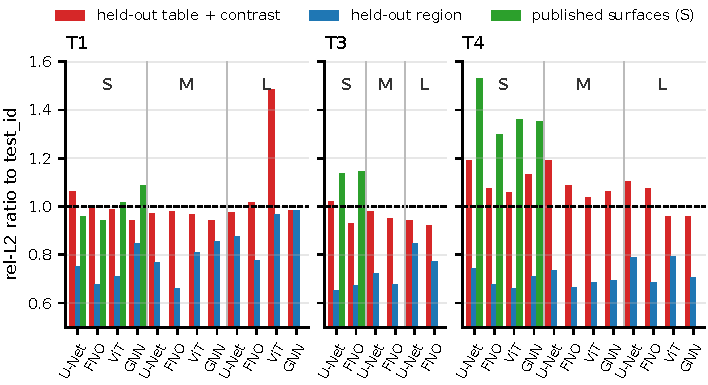
\includegraphics[width=\linewidth]{figA_ood_all.pdf}
  \caption{Per-split OOD degradation for all three tasks (the main-text Figure~\ref{fig:ood} shows T1 and T4).}
  \label{fig:ood_all}
\end{figure}
% src: docs/tables/acceleration.md
\begin{table*}[tb]
\centering
\scriptsize
\setlength{\tabcolsep}{3.5pt}
\caption{Solver acceleration: AMG-preconditioned CG warm-started from the predicted voltage versus a zero start, to a relative residual of $10^{-6}$ (medians over systems; reduction = median of $1 - $ warm/zero per system; warm-start residual = relative Kirchhoff residual of the prediction, zero start = 1). T1V = first pair of each T1 landscape.}
\label{tab:acceleration}
\setlength{\tabcolsep}{2.2pt}
\begin{tabular}{llllrlrlrr}
\toprule
task & tier & model & split & systems & iterations zero $\rightarrow$ warm & reduction & time zero $\rightarrow$ warm (ms) & reduction & warm-start residual \\
\midrule
T1V & L & FNO & test\_id & 1928 & 16 $\rightarrow$ 18 & -7.7 \% & 517.9 $\rightarrow$ 580.5 & -7.5 \% & 34.7 \\
T1V & L & FNO & test\_ood & 1278 & 25 $\rightarrow$ 26 & -7.1 \% & 860.1 $\rightarrow$ 930.0 & -7.3 \% & 91.1 \\
T1V & M & FNO & test\_id & 4823 & 12 $\rightarrow$ 12 & +0.0 \% & 102.5 $\rightarrow$ 105.7 & -4.5 \% & 22.2 \\
T1V & M & FNO & test\_ood & 3225 & 16 $\rightarrow$ 16 & +0.0 \% & 141.3 $\rightarrow$ 143.4 & -1.8 \% & 22.2 \\
T1V & S & FNO & test\_id & 9850 & 9 $\rightarrow$ 10 & +0.0 \% & 23.2 $\rightarrow$ 23.4 & -0.8 \% & 11 \\
T1V & S & FNO & test\_ood & 6460 & 11 $\rightarrow$ 12 & +0.0 \% & 30.2 $\rightarrow$ 30.7 & -0.2 \% & 11.4 \\
T3 & L & FNO & test\_id & 1928 & 17 $\rightarrow$ 18 & -5.6 \% & 757.0 $\rightarrow$ 808.7 & -6.2 \% & 1.62e+03 \\
T3 & L & FNO & test\_ood & 1275 & 23 $\rightarrow$ 24 & -4.2 \% & 1159.8 $\rightarrow$ 1221.1 & -4.4 \% & 1.89e+03 \\
T3 & M & FNO & test\_id & 4823 & 12 $\rightarrow$ 13 & +0.0 \% & 119.9 $\rightarrow$ 120.9 & -0.5 \% & 559 \\
T3 & M & FNO & test\_ood & 3222 & 16 $\rightarrow$ 16 & +0.0 \% & 167.2 $\rightarrow$ 169.3 & -0.5 \% & 653 \\
T3 & S & FNO & test\_id & 9850 & 10 $\rightarrow$ 10 & +0.0 \% & 19.3 $\rightarrow$ 19.7 & -0.1 \% & 181 \\
T3 & S & FNO & test\_ood & 6460 & 11 $\rightarrow$ 11 & +0.0 \% & 25.4 $\rightarrow$ 25.6 & +0.0 \% & 212 \\
T1V & L & U-Net & test\_id & 1928 & 16 $\rightarrow$ 17 & -6.7 \% & 739.5 $\rightarrow$ 821.4 & -7.4 \% & 22.5 \\
T1V & L & U-Net & test\_ood & 1278 & 25 $\rightarrow$ 26 & -5.6 \% & 1248.0 $\rightarrow$ 1320.7 & -5.7 \% & 22.5 \\
T1V & M & U-Net & test\_id & 4823 & 12 $\rightarrow$ 12 & -5.6 \% & 86.9 $\rightarrow$ 91.6 & -6.5 \% & 19.4 \\
T1V & M & U-Net & test\_ood & 3225 & 16 $\rightarrow$ 17 & -4.8 \% & 129.4 $\rightarrow$ 137.6 & -5.7 \% & 17.6 \\
T1V & S & U-Net & test\_id & 9850 & 9 $\rightarrow$ 9 & +0.0 \% & 14.4 $\rightarrow$ 14.4 & +0.0 \% & 5.06 \\
T1V & S & U-Net & test\_ood & 6460 & 11 $\rightarrow$ 11 & +0.0 \% & 19.2 $\rightarrow$ 19.3 & +0.1 \% & 4.69 \\
T3 & L & U-Net & test\_id & 1928 & 17 $\rightarrow$ 19 & -9.1 \% & 763.2 $\rightarrow$ 858.6 & -9.5 \% & 3.32e+03 \\
T3 & L & U-Net & test\_ood & 1275 & 23 $\rightarrow$ 25 & -8.8 \% & 1164.0 $\rightarrow$ 1281.7 & -8.8 \% & 3.87e+03 \\
T3 & M & U-Net & test\_id & 4823 & 12 $\rightarrow$ 13 & -2.9 \% & 99.9 $\rightarrow$ 102.3 & -1.0 \% & 580 \\
T3 & M & U-Net & test\_ood & 3222 & 16 $\rightarrow$ 16 & -4.5 \% & 140.7 $\rightarrow$ 144.5 & -4.5 \% & 783 \\
T3 & S & U-Net & test\_id & 9850 & 10 $\rightarrow$ 10 & +0.0 \% & 19.3 $\rightarrow$ 19.1 & +0.1 \% & 82.5 \\
T3 & S & U-Net & test\_ood & 6460 & 11 $\rightarrow$ 11 & +0.0 \% & 25.4 $\rightarrow$ 24.5 & +0.1 \% & 109 \\
\bottomrule
\end{tabular}
\end{table*}

% src: paper/tables/wp4_data_scaling.md
\begin{table}[tb]
\centering
\small
\setlength{\tabcolsep}{3.5pt}
\caption{Data-scaling ablation at S on T1 (seed 1): training on 1,000 / 5,000 / 20,000 landscapes for 30 epochs or for the official run's number of optimisation steps, against the official run on all training landscapes.}
\label{tab:wp4}
\begin{tabular}{llllllrr}
\toprule
model & n train & regime & rel-L2 & MAE log$_{10}$ & top-5 \% IoU & epochs & GPU-h \\
\midrule
FNO & 1,000 & fixed epochs (30) & 0.575 & 0.255 & 0.416 & 30 & 0.15 \\
FNO & 1,000 & fixed steps & 0.438 & 0.243 & 0.462 & 39 & 0.19 \\
FNO & 5,000 & fixed epochs (30) & 0.357 & 0.180 & 0.577 & 30 & 0.22 \\
FNO & 5,000 & fixed steps & 0.298 & 0.173 & 0.597 & 54 & 0.36 \\
FNO & 20,000 & fixed epochs (30) & 0.243 & 0.137 & 0.665 & 30 & 0.41 \\
FNO & 20,000 & fixed steps & 0.246 & 0.138 & 0.664 & 36 & 0.48 \\
FNO & 61,577 & official run & 0.198 & 0.112 & 0.719 & 29 & 0.95 \\
U-Net & 1,000 & fixed epochs (30) & 0.496 & 0.213 & 0.484 & 30 & 0.17 \\
U-Net & 1,000 & fixed steps & 0.368 & 0.162 & 0.607 & 88 & 0.35 \\
U-Net & 5,000 & fixed epochs (30) & 0.316 & 0.155 & 0.604 & 30 & 0.15 \\
U-Net & 5,000 & fixed steps & 0.139 & 0.076 & 0.818 & 143 & 0.76 \\
U-Net & 20,000 & fixed epochs (30) & 0.188 & 0.072 & 0.771 & 30 & 0.31 \\
U-Net & 20,000 & fixed steps & 0.103 & 0.042 & 0.877 & 94 & 0.94 \\
U-Net & 61,577 & official run & 0.111 & 0.042 & 0.857 & 30 & 0.86 \\
\bottomrule
\end{tabular}
\end{table}


\clearpage
\section{Training and validation curves}
\label{app:curves}

\begin{figure}[h]
  \centering
  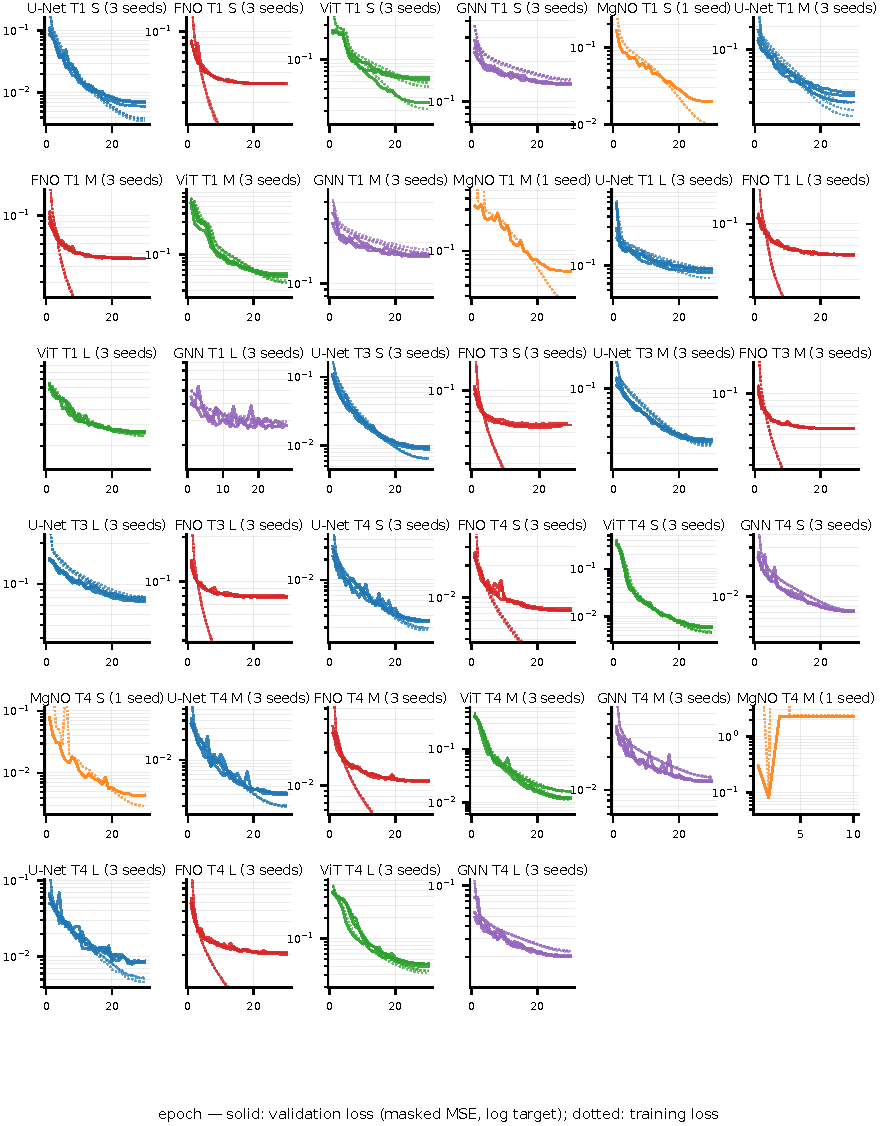
\includegraphics[width=\linewidth]{figA_training_curves.pdf}
  \caption{Training (dotted) and validation (solid) loss per epoch for every official run---one panel per model $\times$ task $\times$ tier, seeds overlaid (masked MSE in the log-target space; early stopping on the validation loss with patience 8; MgNO one seed).}
  \label{fig:curves}
\end{figure}

\begin{figure}[h]
  \centering
  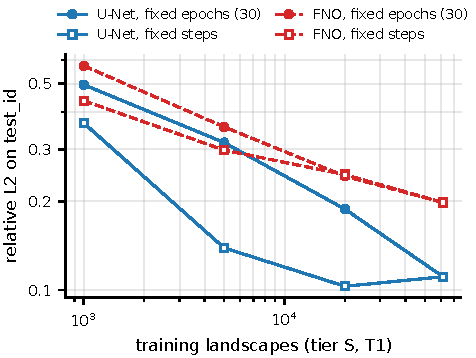
\includegraphics[width=0.48\linewidth]{figA_data_scaling.pdf}
  \caption{Data-scaling ablation at S on T1 (seed 1): relative L2 on \code{test\_id} against the number of training landscapes in the fixed-epoch and fixed-step regimes; the rightmost point of each curve is the official run (Table~\ref{tab:wp4}).}
  \label{fig:scaling}
\end{figure}

\clearpage
\section{Dataset statistics}
\label{app:stats}

Contrast ($\log_{10}$, p10~/ p50~/ p90): synthetic 1.00~/ 3.00~/ 4.00 at every tier with a maximum of $10^6$; real 0.76~/ 1.79~/ 2.79 at S rising to 2.00~/ 3.00~/ 3.00 at XXL with a maximum of $10^3$. Real landscapes cover 14 RESOLVE biomes and 7 realms (largest: Palearctic 16,760 landscapes, Neotropic 15,405, Nearctic 12,005, Australasia 10,470). NoData fraction of real tiles: p50 0.002, p90 0.159, max 0.896.
% src: docs/tables/dataset_statistics.md

\begin{figure}[h]
  \centering
  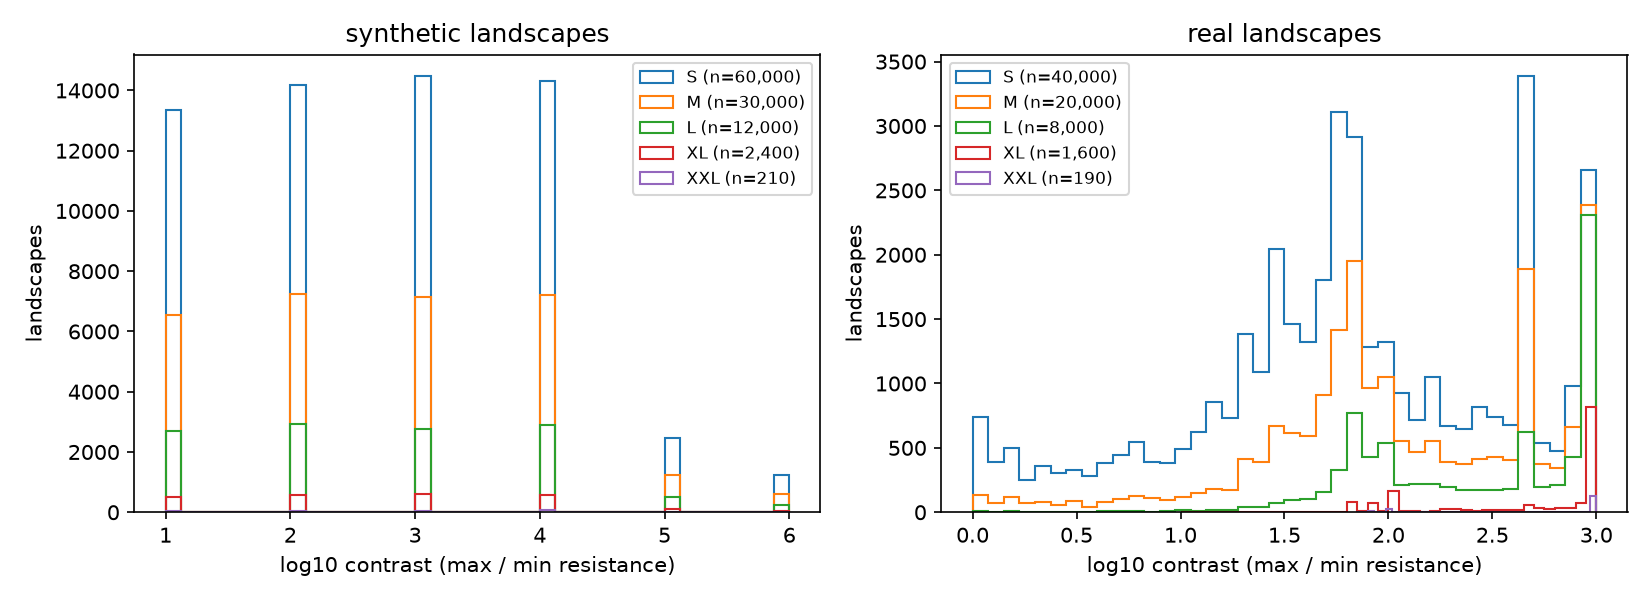
\includegraphics[width=0.48\linewidth]{figA_stats_contrast.png}\hfill
  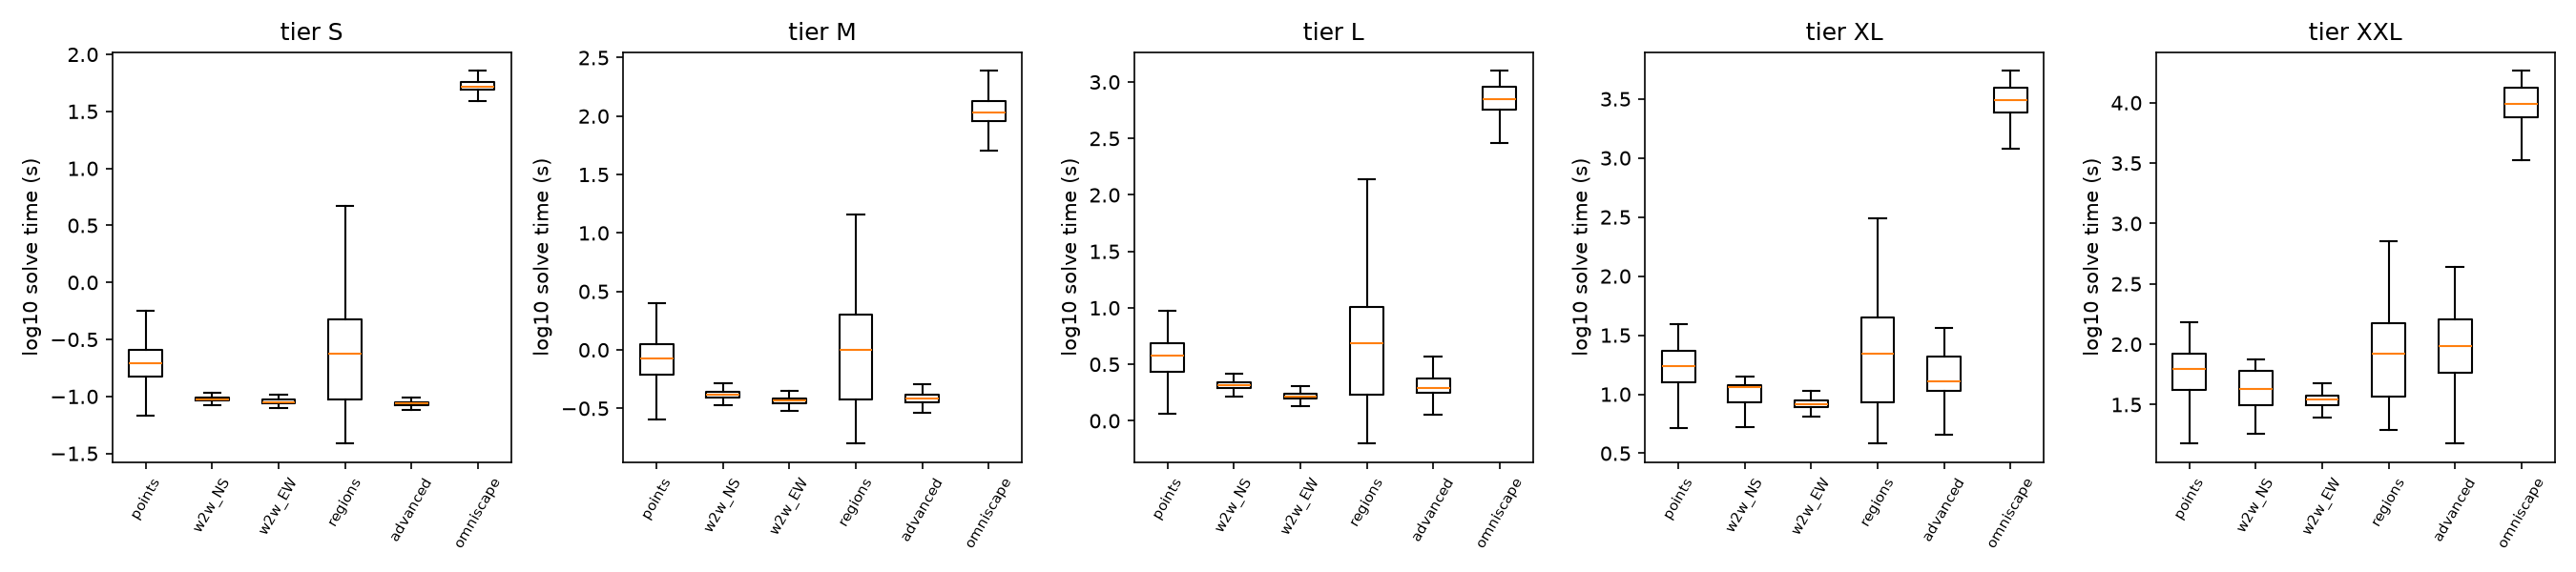
\includegraphics[width=0.48\linewidth]{figA_stats_solve_times.png}\\[2pt]
  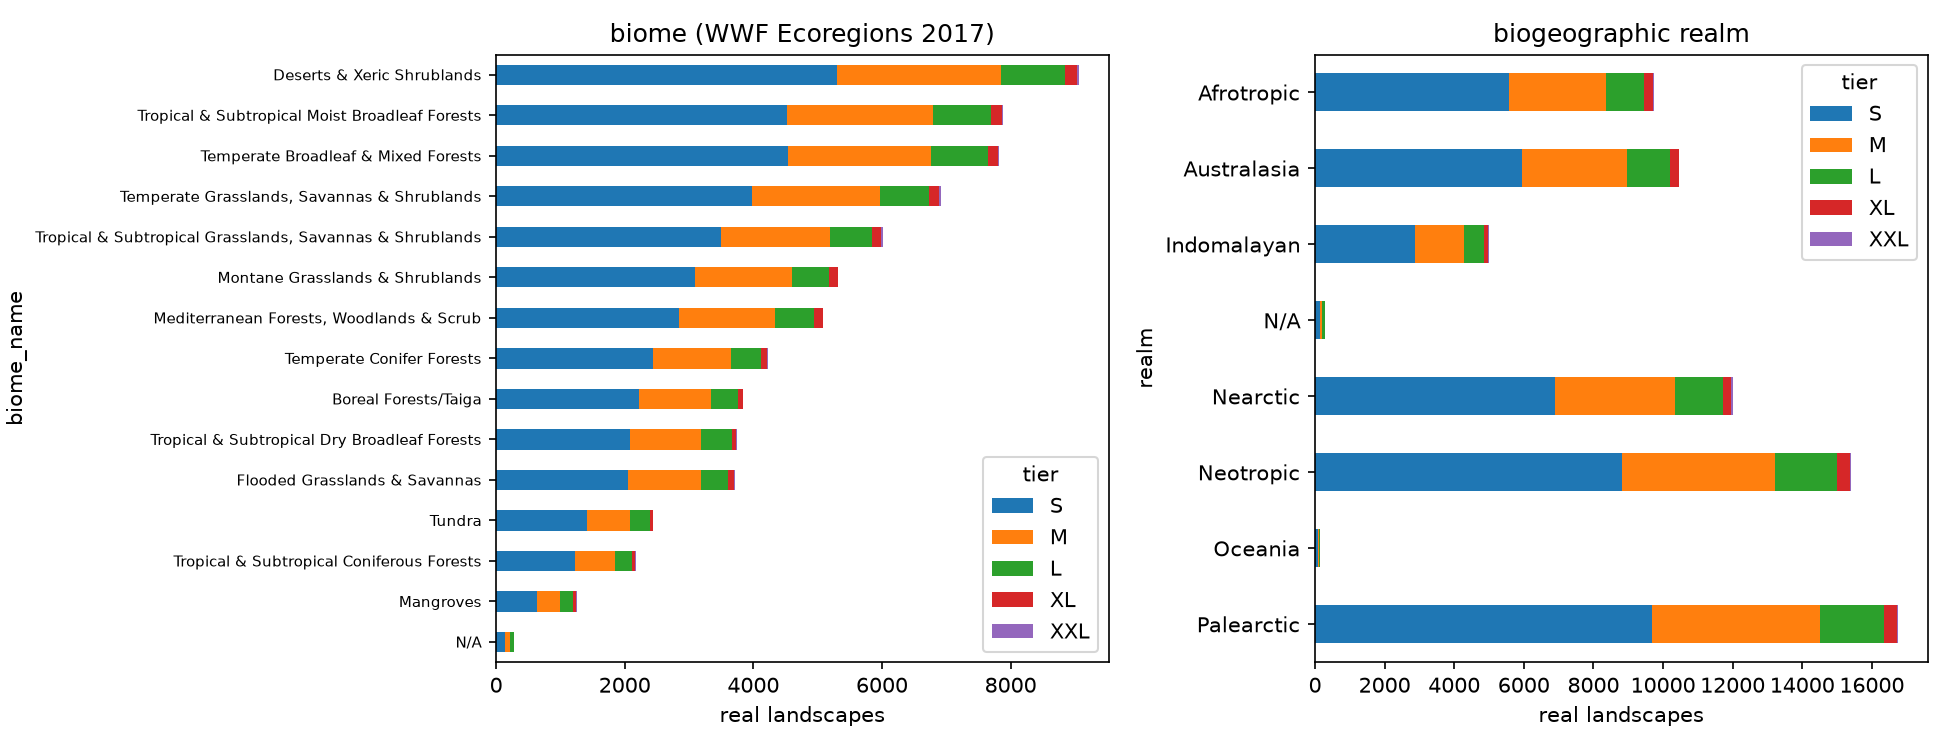
\includegraphics[width=0.48\linewidth]{figA_stats_biome_realm.png}\hfill
  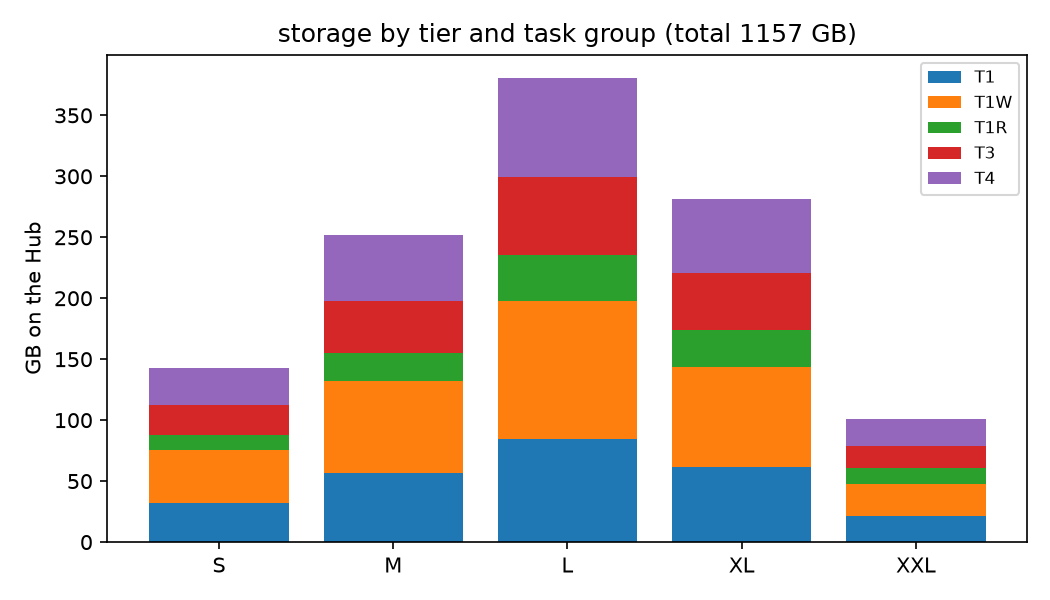
\includegraphics[width=0.48\linewidth]{figA_stats_storage.png}
  \caption{Dataset statistics (v1.0 index): contrast per tier and family, solve time per configuration and tier, biome and realm coverage of the real landscapes, and storage per tier and task group.}
  \label{fig:stats}
\end{figure}

% src: docs/tables/final_counts.json
\begin{table}[tb]
\centering
\small
\setlength{\tabcolsep}{3.5pt}
\caption{Landscapes per split and tier (index counts before QC exclusion; XL after the v1.0.2 correction of amendment C3).}
\label{tab:splits}
\begin{tabular}{lrrrrrr}
\toprule
tier & train & val & test\_id & test\_ood & ood\_region & QC-failing landscapes \\
\midrule
S & 63,303 & 10,917 & 9,850 & 6,460 & 9,470 & 1 \\
M & 31,496 & 5,651 & 4,823 & 3,225 & 4,805 & 4 \\
L & 12,613 & 2,235 & 1,928 & 1,279 & 1,945 & 10 \\
XL & 880 & 131 & 2,335 & 254 & 400 & 7 \\
XXL & 0 & 0 & 275 & 25 & 100 & 2 \\
\bottomrule
\end{tabular}
\end{table}


\clearpage
\section{Omniscape fidelity}
\label{app:fidelity}

The block rule (block = largest odd integer $\le$ radius/10) came from a 3-sample-per-cell study against the exact block-1 map: block 3 at S deviated by 4.49\,\% mean~/ 7.60\,\% max relative L2 and block 5 at M by 2.00\,\%~/ 2.45\,\%, while coarsening XL 17$\rightarrow$33 changed the cumulative current by 2.47\,\%~/ 2.93\,\% and XXL 33$\rightarrow$65 by 9.46\,\%~/ 11.85\,\% (both rejected); block 1 was 6.4$\times$ (S) and 22.6$\times$ (M) more expensive at those anchors. The $\approx 1$\,\% target was an extrapolation and proved optimistic: the production M block deviates from the exact map by 3.1\,\% relative L2 on average on 200 synthetic test/OOD landscapes (median 2.8\,\%, top-5\,\% IoU 0.95, pinch-point recall 0.95), and the full 1\,000-sample M reference gives mean \relltwo{} 0.029 (median 0.027) with 4.7\,\% of samples above 5\,\% (11\,\% of synthetic, 1.4\,\% of real tiles; real tiles never above 8\,\%). At L (block 5, 60 samples) the mean is 0.028 (max 0.058; 2 of 60 above 5\,\%); block 1 costs 6.7$\times$ (M) and 22$\times$ (L) the production solve. T4 rows carry no single residual; each window solve is bounded by Circuitscape's enforced relative residual $\le 10^{-4}$, with a rescue path for the contrast-$10^6$ solves that the stock package aborts.
% src: docs/t4_fidelity.md; docs/dataset_card.md

\begin{figure}[h]
  \centering
  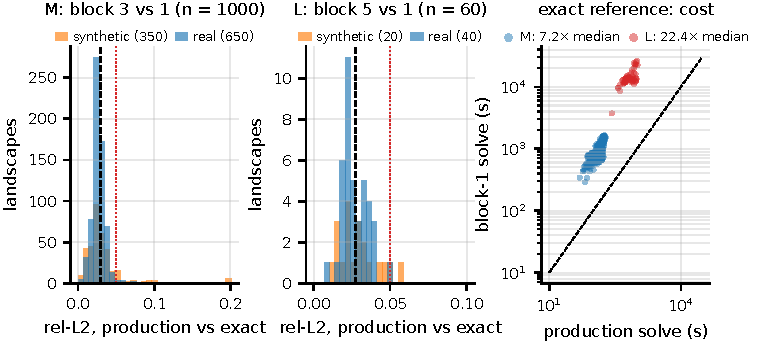
\includegraphics[width=\linewidth]{figA_fidelity.pdf}
  \caption{Fidelity of the production T4 targets on the reference subsets: per-landscape \relltwo{} of the production block against the exact block-1 map at M and L (dashed: mean; dotted: the 5\,\% tail threshold), and the solve-time cost of the exact reference against the production solve.}
  \label{fig:fidelity}
\end{figure}

\section{Precision pass}
\label{app:precision}

% src: docs/tables/precision_pass.md
\begin{table*}[tb]
\centering
\scriptsize
\setlength{\tabcolsep}{3.5pt}
\caption{Post-run precision pass per tier: every T1/T1W/T1R/T3 row above $10^{-9}$, unmeasured, CG+AMG-solved or QC-failed was re-solved with CHOLMOD on the reduced system plus up to three refinement steps; rows that cannot reach $10^{-6}$ in double precision are flagged and excluded from the split lists.}
\label{tab:precision}
\setlength{\tabcolsep}{2.2pt}
\begin{tabular}{lrrlrr}
\toprule
tier & rows re-solved & CG+AMG $\rightarrow$ CHOLMOD & residual after: p50 / p90 / p99 / max & rows $> 10^{-9}$ & rows $> 10^{-6}$ (flagged) \\
\midrule
S & 68,008 & 9 & 2.9e-13 / 3.4e-11 / 1.6e-09 / 5.0e-07 & 1,013 & 0 \\
M & 37,639 & 14 & 9.1e-13 / 1.9e-10 / 5.2e-09 / 1.4e-06 & 1,136 & 4 \\
L & 18,691 & 110 & 6.8e-12 / 4.9e-10 / 1.4e-08 / 1.5e-05 & 1,014 & 9 \\
XL & 4,774 & 47 & 6.9e-11 / 1.3e-09 / 4.3e-08 / 6.6e-06 & 551 & 5 \\
XXL & 610 & 9 & 2.7e-10 / 4.3e-09 / 2.0e-07 / 4.0e-05 & 147 & 2 \\
total & 129,722 & 189 &  & 3,861 & 20 \\
\bottomrule
\end{tabular}
\end{table*}


\begin{figure}[h]
  \centering
  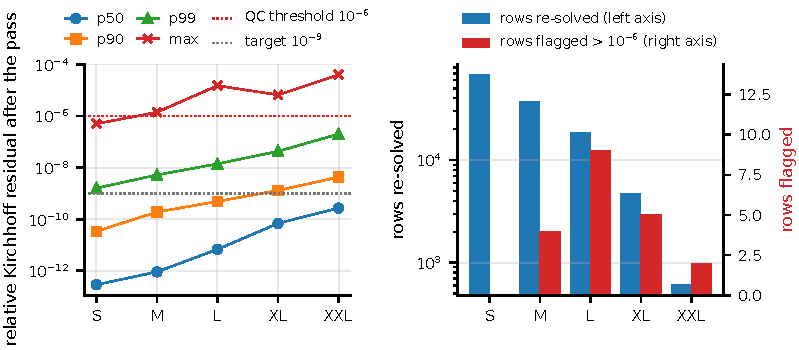
\includegraphics[width=\linewidth]{figA_precision.pdf}
  \caption{The post-run precision pass per tier: quantiles of the relative Kirchhoff residual after the pass against the QC threshold ($10^{-6}$) and the target ($10^{-9}$), and the number of rows re-solved and flagged.}
  \label{fig:precision}
\end{figure}

Generation ran from 2026-09-16 to 2026-09-22 followed by a 29~h precision pass, 16\,552 core-hours in all (generation 14\,379, precision pass 1\,249, audits 30, auxiliary sets and probes 893); the eleven operational incidents and their resolutions are in the post-mortem.
% src: docs/generation_postmortem.md

\clearpage
\section{Many-query demonstration, per tile}
\label{app:wp7}

\begin{figure}[h]
  \centering
  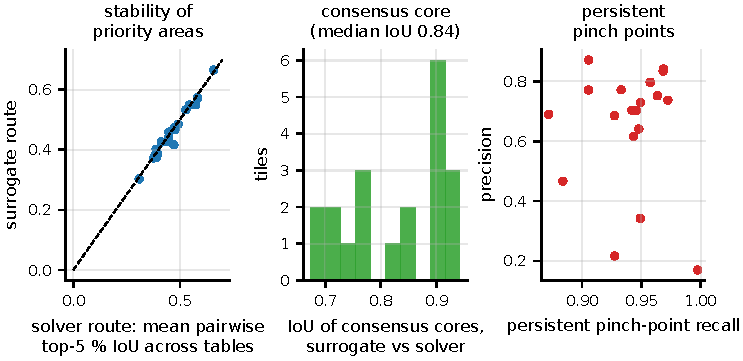
\includegraphics[width=\linewidth]{figA_wp7.pdf}
  \caption{Per-tile agreement between the solver route and the surrogate route in the many-query demonstration (20 real L tiles $\times$ 8 resistance tables): stability of the top-5\,\% regions across tables, consensus-core overlap and persistent pinch-point recall/precision.}
  \label{fig:wp7}
\end{figure}

\section{Splits per tier}
\label{app:splits}
The per-tier split counts are in Table~\ref{tab:splits} (Appendix~\ref{app:stats}); subset sizes and the QC exclusion rule are in Section~\ref{sec:data}.

\section{Evaluation CLI and prediction format}
\label{app:format}

\code{python scripts/evaluate.py --predictions <dir> --split <name>[,<name>] [--root <data root> --tier <tier> --subset <name> --out <dir> --acceleration --t4-reference <aux build> --t4-blocks <builds> --workers <n>]} writes \code{results.json} and \code{results.md}. \code{<dir>/predictions.h5} holds one group per sample and one subgroup per configuration with \code{cum\_current} (float32 $H\times W$; T1, T1W, T1R, T4), optional \code{voltage} (float32 $H\times W$ or $P\times H\times W$), optional \code{pairwise\_current} ($P\times H\times W$), \code{reff} (float64 $K\times K$; T2), \code{current} (float32 $H\times W$; T3) and optional \code{flow\_potential}~/ \code{normalized} (T4), plus a group attribute \code{inference\_time\_s} per configuration (wall clock including preprocessing); \code{<dir>/meta.json} records model, task, tier, split, seed and notes. Only \code{qc\_pass} rows of the requested splits are evaluated, samples absent from the file are skipped with the row count reported, processing is deterministic in sorted order, an oracle scores 0 error~/ 1.0 on every similarity metric and an all-zero predictor scores \relltwo{} = 1 and top-$q$ IoU = 0. The leaderboard entry schema, the validator and the submission procedure are in \code{docs/submission.md}.
% src: scripts/evaluate.py; ampscape/eval/harness.py; docs/evaluation.md

\section{Licences and attributions}
\label{app:licences}

% src: docs/licenses.md
\begin{table*}[tb]
\centering
\scriptsize
\setlength{\tabcolsep}{3.5pt}
\caption{Upstream data sources, their licences and what AmpScape stores (derived rasters only; never the source tiles). WDPA polygons (restrictive licence) and OpenStreetMap (ODbL) are not used. The dataset is released under CC BY 4.0, code and solver wrapper under MIT.}
\label{tab:licences}
\resizebox{\textwidth}{!}{%
\begin{tabular}{p{3.0cm}p{3.0cm}p{5.2cm}p{3.0cm}}
\toprule
layer & version & licence & derived rasters redistributed \\
\midrule
ESA WorldCover land cover, 10 m & 2021 v200 & CC BY 4.0 & class codes \\
Copernicus DEM GLO-30 & 2021 release (DLR 2010--2014, Airbus 2014--2018) & Copernicus licence; Art. 4 rights of use, Art. 6 notices reproduced & elevation, slope \\
GRIP4 global roads & v4, 2018 & CC0 by the publisher; CC BY 4.0 in secondary catalogues (attributed as CC BY 4.0) & distance-to-road only \\
HydroRIVERS & v1.0 & CC BY 4.0 & distance-to-river only \\
gHM global Human Modification & v1, 1 km & CC BY 4.0 & gHM \\
RESOLVE Ecoregions 2017 & 2017 & CC BY 4.0 & stratification only (biome, realm) \\
Eurac Alps permeability & 2022 & CC BY 4.0 & published resistance tiles \\
Hawaiian gallinule resistance & 2020 & CC0 1.0 & published resistance tiles \\
Northern raccoon Europe maps & 2025 & CC BY 4.0 & published resistance tiles \\
\bottomrule
\end{tabular}}
\end{table*}


Every file in the source manifest (21 entries, 5.45~GB) has a recorded licence and sha256, enforced by \code{tests/test\_licenses.py}. The dataset is released under CC BY 4.0; code and the solver wrapper under MIT; Circuitscape.jl 5.17.1 and Omniscape.jl 0.6.2 are MIT. The full attribution block and the Copernicus notices are reproduced in the dataset card and \code{LICENSE-DATA}.
% src: docs/licenses.md; docs/dataset_card.md

\clearpage
\section*{NeurIPS Paper Checklist}

\begin{enumerate}
\item {\bf Claims}\\
    Question: Do the main claims made in the abstract and introduction accurately reflect the paper's contributions and scope?\\
    Answer: \answerYes{}\\
    Justification: The abstract and Section~1 state the dataset, the protocol, the harness, the baselines and the demonstration; every number quoted is from the tables of Section~7 and Appendix~B, and the scope (``a trade-off, not a replacement'') matches the results.
\item {\bf Limitations}\\
    Question: Does the paper discuss the limitations of the work performed by the authors?\\
    Answer: \answerYes{}\\
    Justification: Section~9 lists nine limitations and the claims the paper does not make.
\item {\bf Theory assumptions and proofs}\\
    Question: For each theoretical result, does the paper provide the full set of assumptions and a complete (and correct) proof?\\
    Answer: \answerYes{}\\
    Justification: The only derivation (the zero-shot scale-transfer error, Appendix~A) states its assumptions and scope.
\item {\bf Experimental result reproducibility}\\
    Question: Does the paper fully disclose all the information needed to reproduce the main experimental results of the paper to the extent that it affects the main claims and/or conclusions of the paper?\\
    Answer: \answerYes{}\\
    Justification: Sections~6 and 7 give the protocol; the repository contains the training, transfer and evaluation scripts, the locked environment and the configuration files; the results are regenerated from the published result files by two scripts named in Section~9.
\item {\bf Open access to data and code}\\
    Question: Does the paper provide open access to the data and code, with sufficient instructions to faithfully reproduce the main experimental results?\\
    Answer: \answerYes{}\\
    Justification: Data on the Hugging Face Hub (CC BY 4.0) with Croissant metadata and a \code{mini} sample; code (MIT) with a README quickstart, the exact evaluation command (Appendix~H) and the leaderboard tooling; anonymised at submission.
\item {\bf Experimental setting/details}\\
    Question: Does the paper specify all the training and test details necessary to understand the results?\\
    Answer: \answerYes{}\\
    Justification: Section~7 (models, epochs, optimiser, patience, seeds, normalisation, configuration selection on validation loss), Appendix~B (per-task decisions) and Appendix~C (training curves).
\item {\bf Experiment statistical significance}\\
    Question: Does the paper report error bars suitably and correctly defined or other appropriate information about the statistical significance of the experiments?\\
    Answer: \answerYes{}\\
    Justification: Every official result is mean $\pm$ sample standard deviation over three training seeds (1-sigma), with the median over seeds for \relltwo{} (Section~6 explains why); single-seed studies are marked as such.
\item {\bf Experiments compute resources}\\
    Question: For each experiment, does the paper provide sufficient information on the computer resources needed to reproduce the experiments?\\
    Answer: \answerYes{}\\
    Justification: Section~9 (701.5 GPU-hours over 773 jobs on L40S, A100, H100 and H200 GPUs; 16\,552 CPU core-hours for generation), Table~\ref{tab:baselines_full} (GPU-hours per run) and Appendix~F (generation breakdown); the total includes abandoned and duplicate runs.
    % src: docs/tables/gpu_usage.md; docs/generation_postmortem.md
\item {\bf Code of ethics}\\
    Question: Does the research conducted in the paper conform, in every respect, with the NeurIPS Code of Ethics?\\
    Answer: \answerYes{}\\
    Justification: No human subjects, no personal data; licences of every source respected (Appendix~I).
\item {\bf Broader impacts}\\
    Question: Does the paper discuss both potential positive societal impacts and negative societal impacts of the work performed?\\
    Answer: \answerYes{}\\
    Justification: Section~9: intended use is screening, not final decisions; a faster approximation does not reduce resistance-surface uncertainty; surrogates must be solver-verified before a decision map.
\item {\bf Safeguards}\\
    Question: Does the paper describe safeguards that have been put in place for responsible release of data or models that have a high risk for misuse?\\
    Answer: \answerNA{}\\
    Justification: Solver outputs on synthetic and open-data landscapes; no high-risk model is released.
\item {\bf Licenses for existing assets}\\
    Question: Are the creators or original owners of assets used in the paper properly credited and are the license and terms of use explicitly mentioned and properly respected?\\
    Answer: \answerYes{}\\
    Justification: Appendix~I lists every upstream layer with version and licence; the solvers and the vendored MgNO code are MIT and cited.
\item {\bf New assets}\\
    Question: Are new assets introduced in the paper well documented and is the documentation provided alongside the assets?\\
    Answer: \answerYes{}\\
    Justification: Dataset card (datasheet), Croissant file with RAI fields, licence, limitations and maintenance plan on the Hub; code documented in the repository.
\item {\bf Crowdsourcing and research with human subjects}\\
    Question: For crowdsourcing experiments and research with human subjects, does the paper include the full text of instructions given to participants and screenshots, if applicable, as well as details about compensation (if any)?\\
    Answer: \answerNA{}\\
    Justification: No human subjects.
\item {\bf Institutional review board (IRB) approvals or equivalent for research with human subjects}\\
    Question: Does the paper describe potential risks incurred by study participants, whether such risks were disclosed to the subjects, and whether Institutional Review Board (IRB) approvals (or an equivalent approval/review based on the requirements of your country or institution) were obtained?\\
    Answer: \answerNA{}\\
    Justification: No human subjects.
\item {\bf Declaration of LLM usage}\\
    Question: Does the paper describe the usage of LLMs if it is an important, original, or non-standard component of the core methods in this research?\\
    Answer: \answerNA{}\\
    Justification: LLMs were used for writing and code assistance only; they are not part of the dataset, the solvers or the baselines.
\end{enumerate}

\end{document}
